%Appendix A


\section{Appendix}
\label{AppendixA}

All numerical calculations were written and performed in Python.

\subsection{Cavity Angle and Polar Angle Relation}

\begin{figure}[H]
	\centering
	\captionsetup{justification = raggedright}
	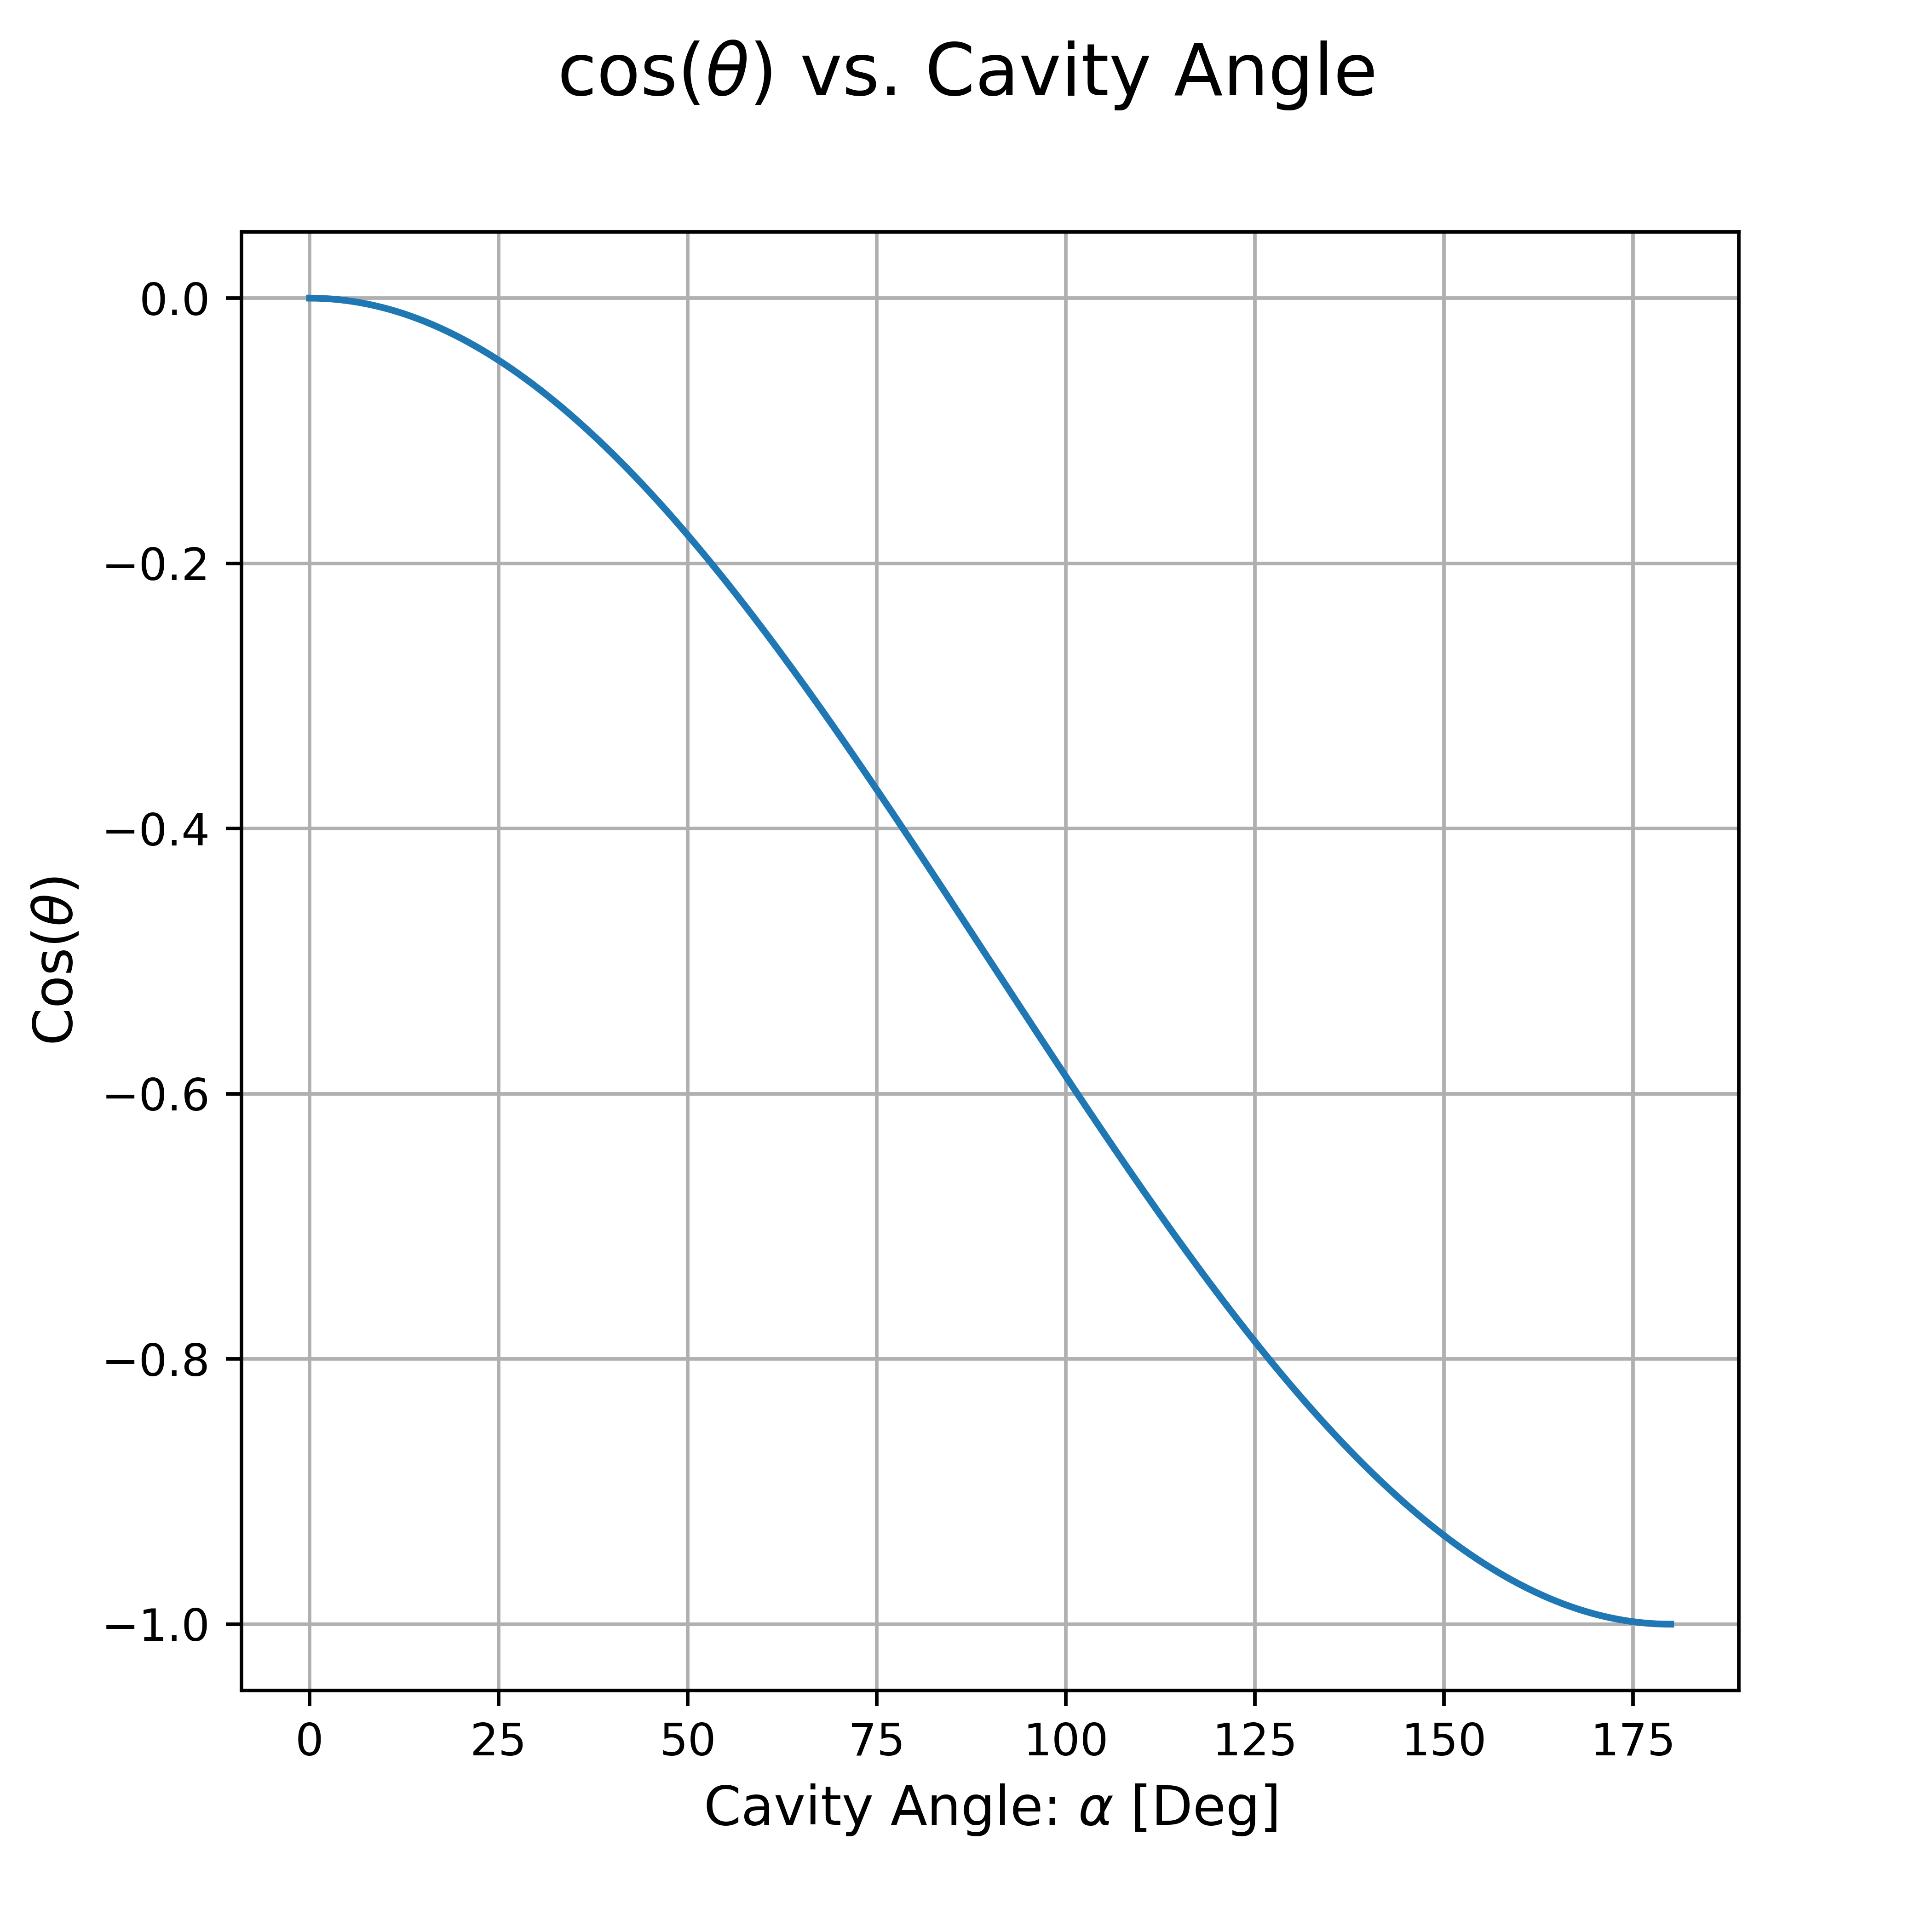
\includegraphics[width=0.4\textwidth]{Graphs/ThetaAlpha.png}
	\caption{Relation between $\cos(\theta)$ and cavity angle $\alpha$ when spherical symmetry is present}
	\label{ThetaAlpha}
\end{figure}


\subsection{Amplitude and Polar Angle Measurement Tables}
For clarity, instead of plotting $\cos(\theta)$ we plot $|\cos(\theta)|$ since cosine is symmetric about $\theta = 0$.

\begin{multicols}{2}
	\begin{table}[H]
		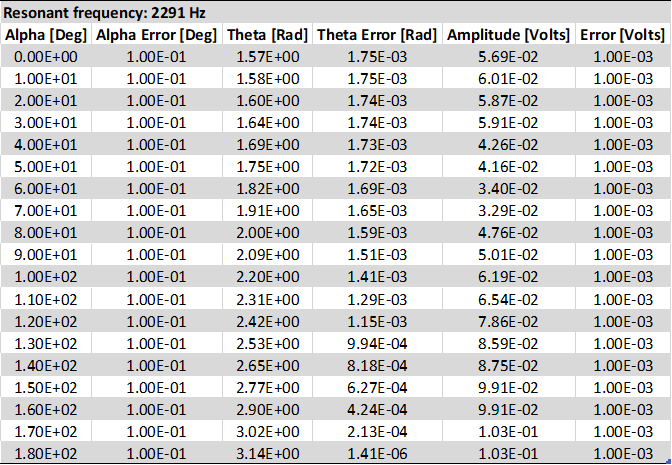
\includegraphics[width=0.45\textwidth]{Tables/2291Table.png}
		\caption{Data table for resonant frequency $2291$ Hz.}
		\label{2291Table}		
	\end{table} 
	\columnbreak
	\begin{figure}[H]
		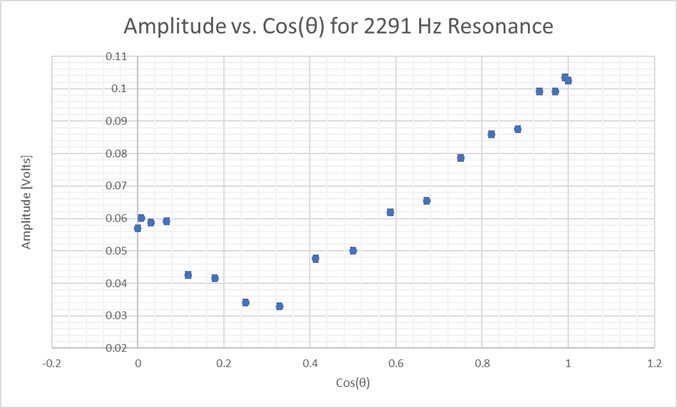
\includegraphics[width=0.45\textwidth]{Graphs/2291Graph.png}
		\caption{Graph of \cref{2291Table}. We can clearly see a single node at $\theta = 1.91$ radians.}
		\label{2291Graph}
	\end{figure}
\end{multicols}

\pagebreak

\begin{multicols}{2}
	\begin{table}[H]
		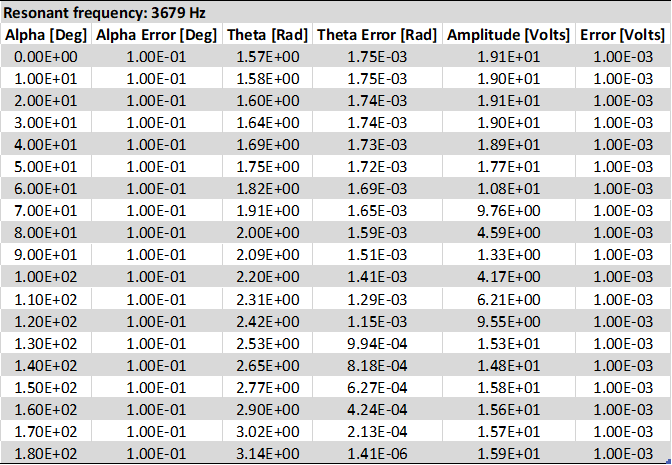
\includegraphics[width=0.45\textwidth]{Tables/3679Table.png}
		\caption{Table showing amplitude vs polar angle for 3679 Hz resonance.}
		\label{3679Table}		
	\end{table} 
	\columnbreak
	\begin{figure}[H]
		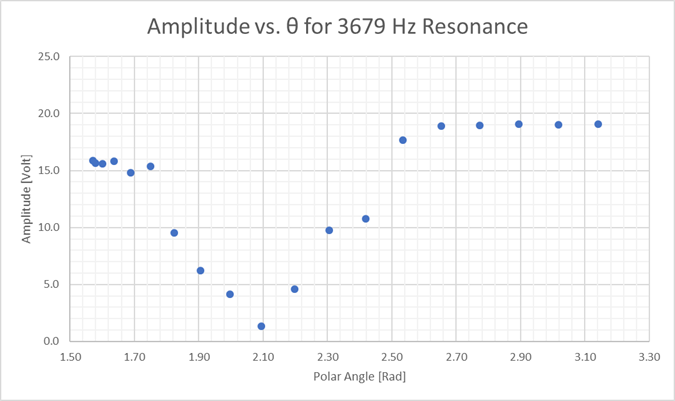
\includegraphics[width=0.45\textwidth]{Graphs/3679Graph.png}
		\caption{Graph of \cref{3679Table}. We can clearly see a single node at $\theta = 2.09$ radians.}
		\label{3679Graph}
	\end{figure}
\end{multicols}



\begin{multicols}{2}	
	\begin{table}[H]
		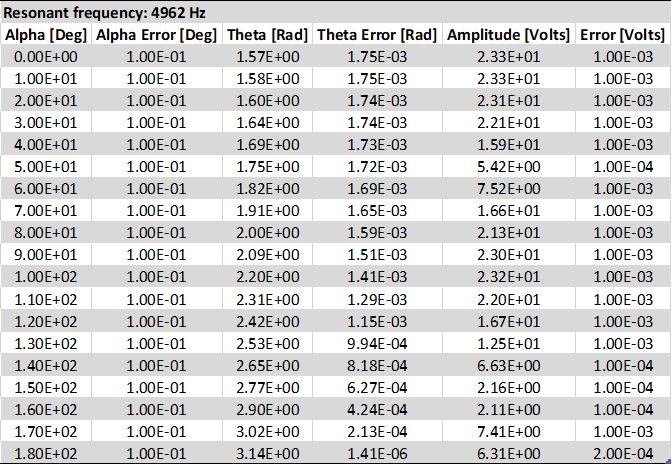
\includegraphics[width=0.45\textwidth]{Tables/4962Table.png}
		\caption{Table showing amplitude vs polar angle for 4926 Hz resonance.}
		\label{4962Table}		
	\end{table}
	\columnbreak
	\begin{figure}[H]
		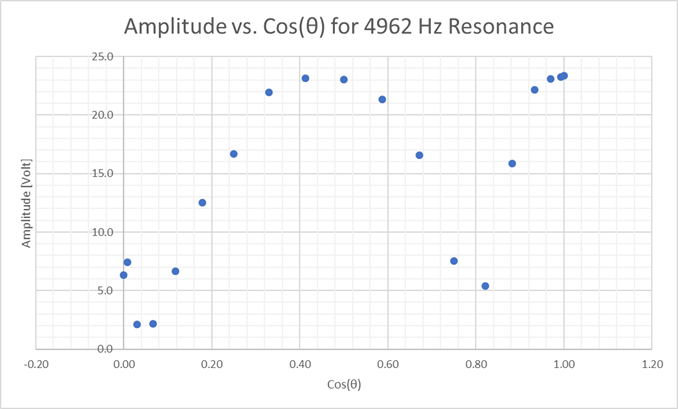
\includegraphics[width=0.45\textwidth]{Graphs/4962Graph.png}
		\caption{Graph of \cref{4962Table}. We can clearly see a single node at $\theta = $ radians.}
		\label{4962Graph}
	\end{figure}
\end{multicols}


\begin{multicols}{2}	
	\begin{table}[H]
		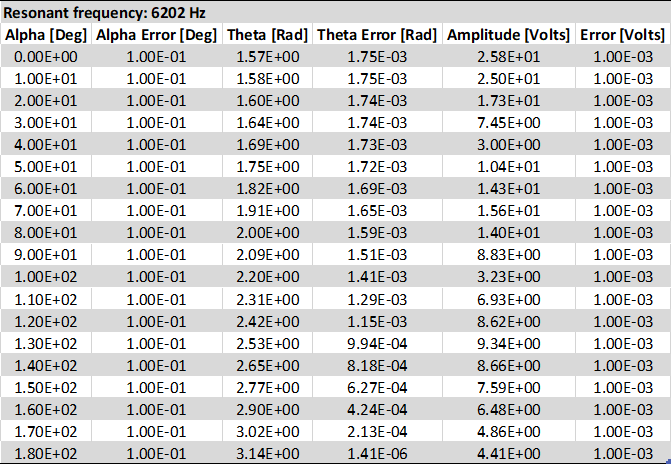
\includegraphics[width=0.45\textwidth]{Tables/6202Table.png}
		\caption{Table showing amplitude vs polar angle for 6202 Hz resonance.}
		\label{6202Table}		
	\end{table}
	\columnbreak
	\begin{figure}[H]
		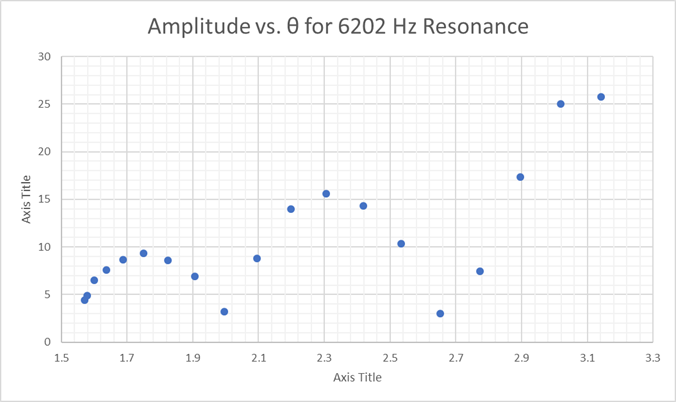
\includegraphics[width=0.45\textwidth]{Graphs/6202Graph.png}
		\caption{Graph of \cref{6202Table}. We can clearly see a single node at $\theta = $ radians.}
		\label{6202Graph}
	\end{figure}
\end{multicols}

\pagebreak

\begin{multicols}{2}	
	\begin{table}[H]
		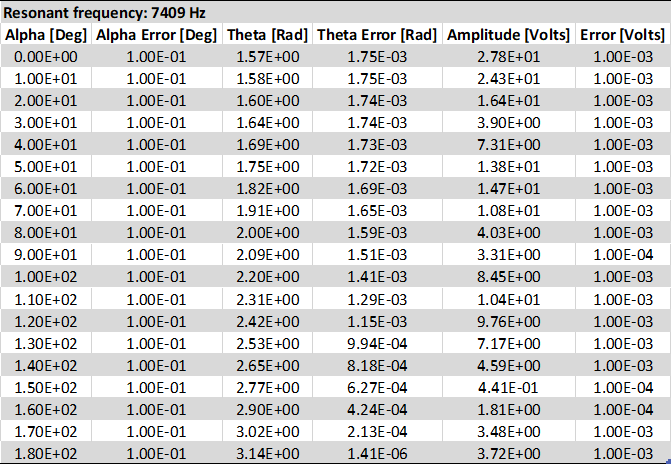
\includegraphics[width=0.45\textwidth]{Tables/7409Table.png}
		\caption{Table showing amplitude vs polar angle for 7409 Hz resonance.}
		\label{7409Table}		
	\end{table}
	\columnbreak
	\begin{figure}[H]
		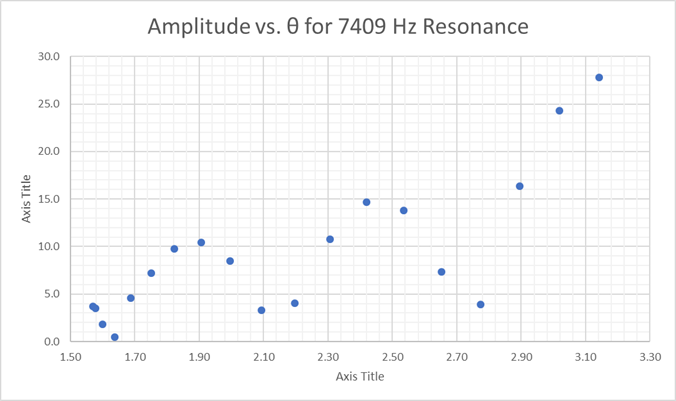
\includegraphics[width=0.45\textwidth]{Graphs/7409Graph.png}
		\caption{Graph of \cref{7409Table}. We can clearly see a single node at $\theta = $ radians.}
		\label{7409Graph}
	\end{figure}
\end{multicols}


\subsection{Legender Polynomial Comparisons}
\begin{figure}[H]
	\centering
	\subfloat[Measured acoustic amplitude plotted against $\cos(\theta)$ for the 2291 Hz resonance]{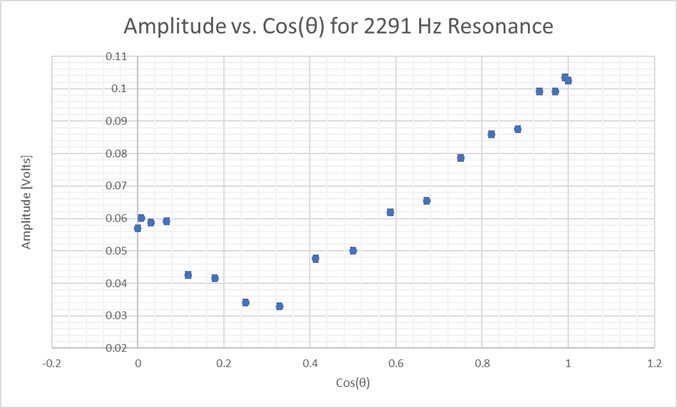
\includegraphics[height=6cm]{Graphs/2291Graph.png}}
	\qquad
	\subfloat[Legendre polynomial $|\mathrm{P}_1|^2$]{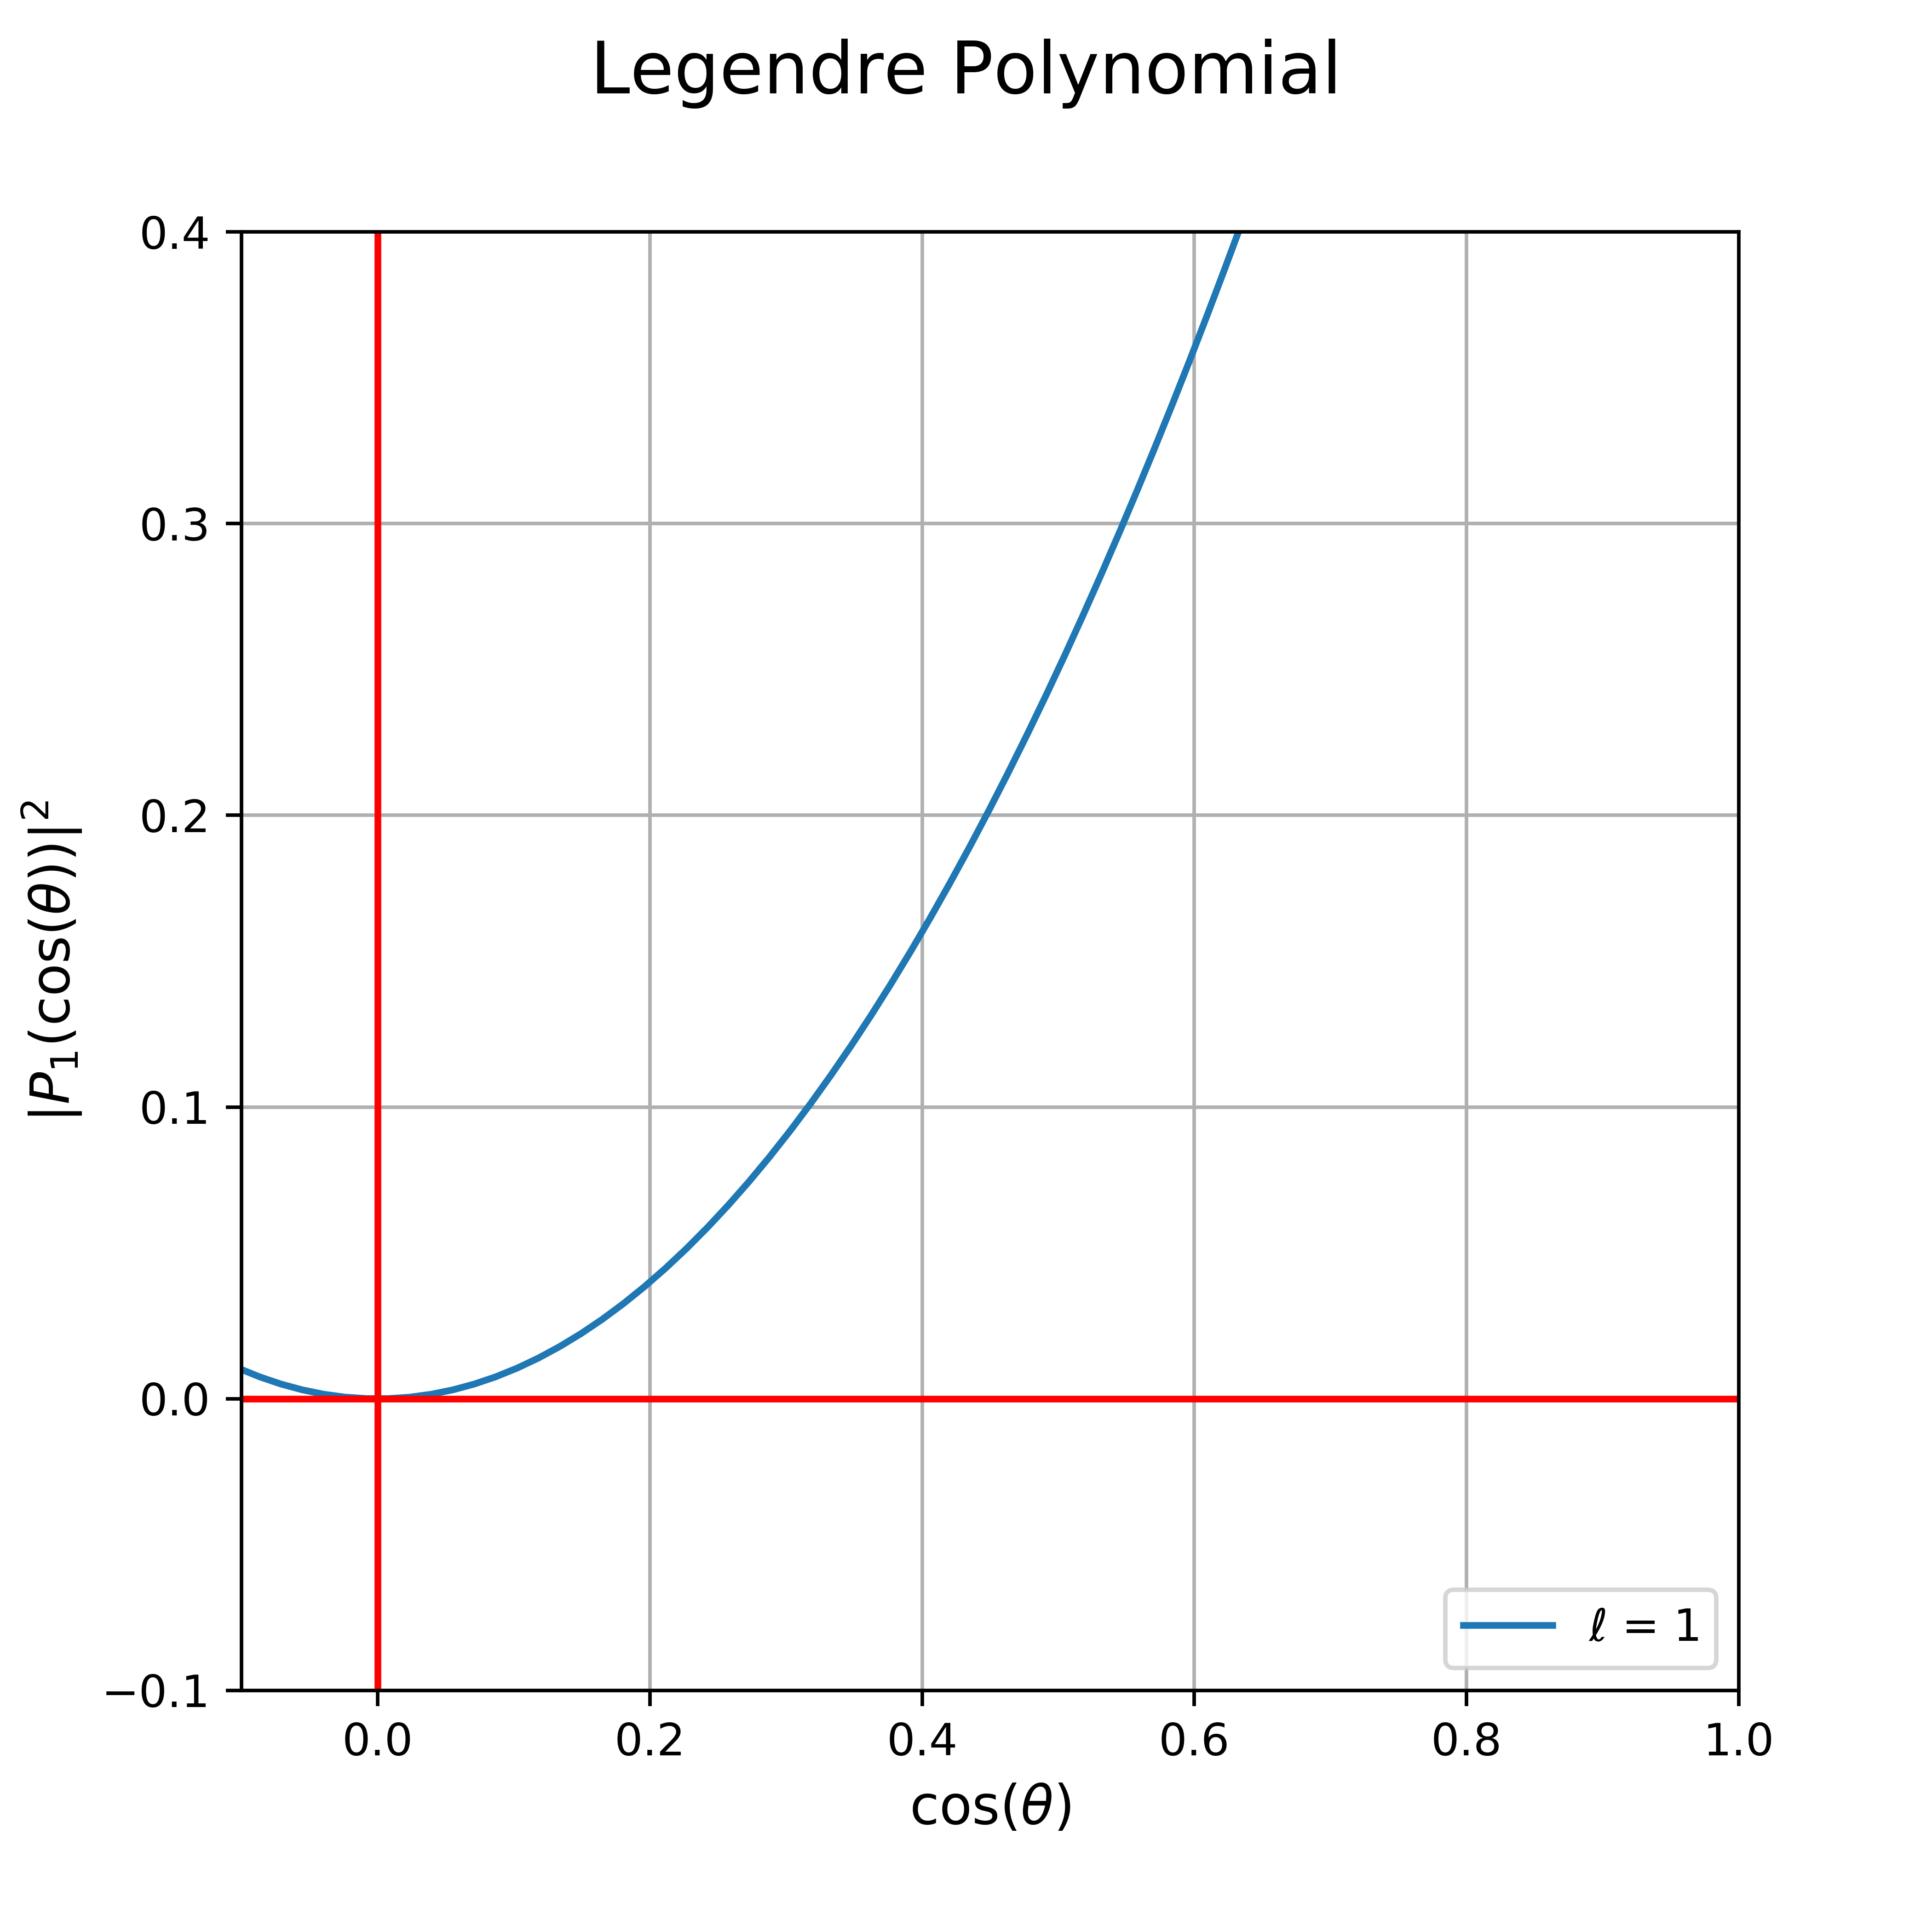
\includegraphics[height=6cm]{Legendre/legendreL1.png}\label{L1}}
	\caption{Comparison of the measured data and the $\ell=1$ Legendre polynomial for the $2291$ Hz resonance.}
	\label{legendre1}
\end{figure}

\begin{figure}[H]
	\centering
	\subfloat[Measured acoustic amplitude plotted against $\cos(\theta)$ for the 3679 Hz resonance]{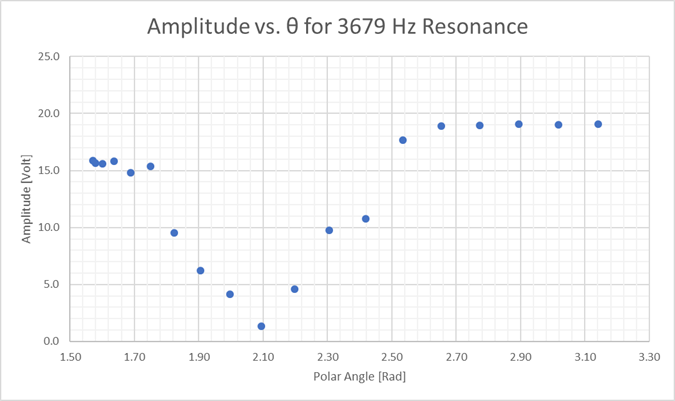
\includegraphics[height=6cm]{Graphs/3679Graph.png}}
	\qquad
	\subfloat[Legendre polynomial $|\mathrm{P}_2|^2$]{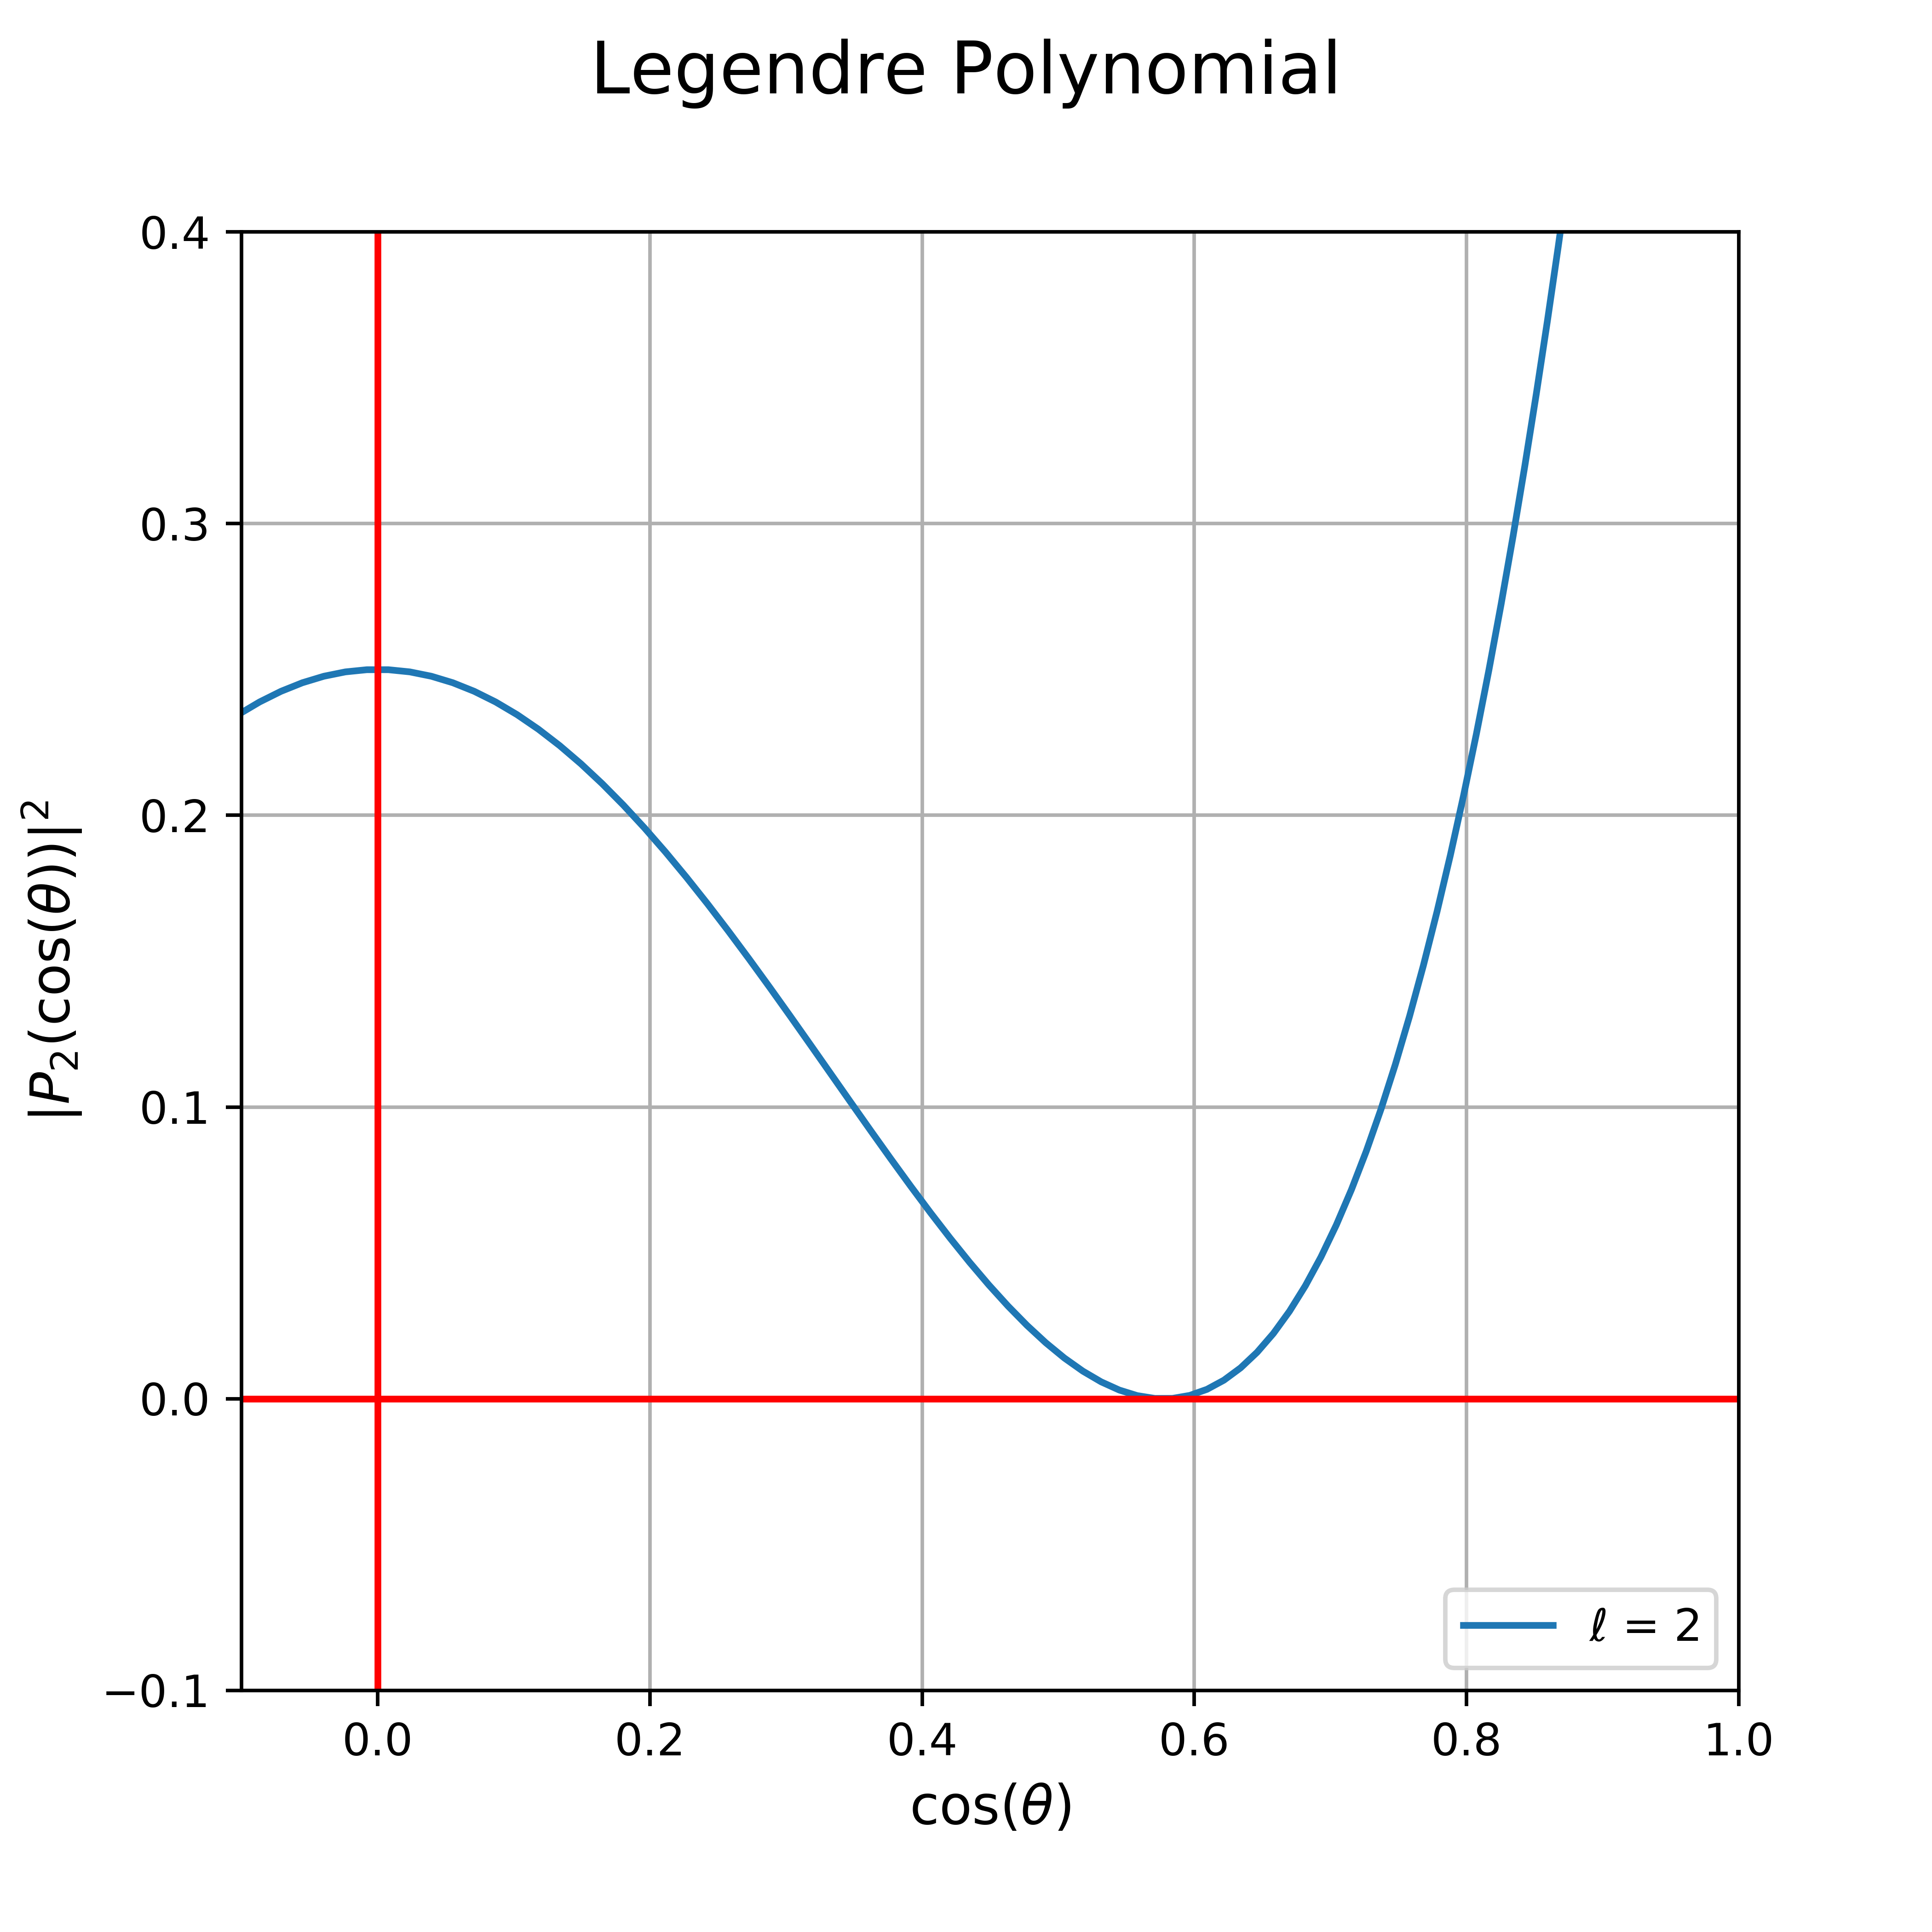
\includegraphics[height=6cm]{Legendre/legendreL2.png}\label{L2}}
	\caption{Comparison of the measured data and the $\ell=2$ Legendre polynomial for the $3679$ Hz resonance.}
	\label{legendre2}
\end{figure}

\begin{figure}[H]
	\centering
	\subfloat[Measured acoustic amplitude plotted against $\cos(\theta)$ for the 4962 Hz resonance]{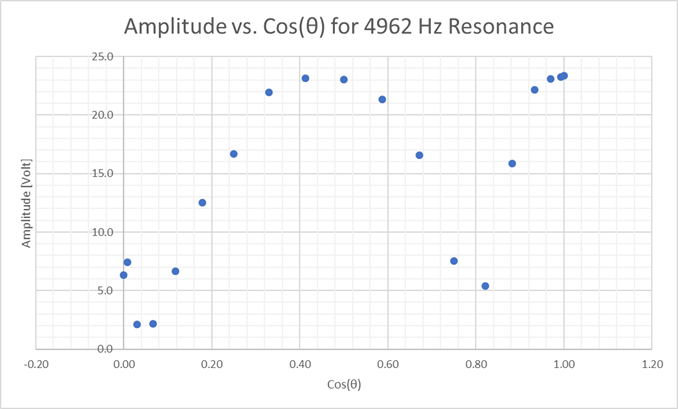
\includegraphics[height=6cm]{Graphs/4962Graph.png}}
	\qquad
	\subfloat[Legendre polynomial $|\mathrm{P}_3|^2$]{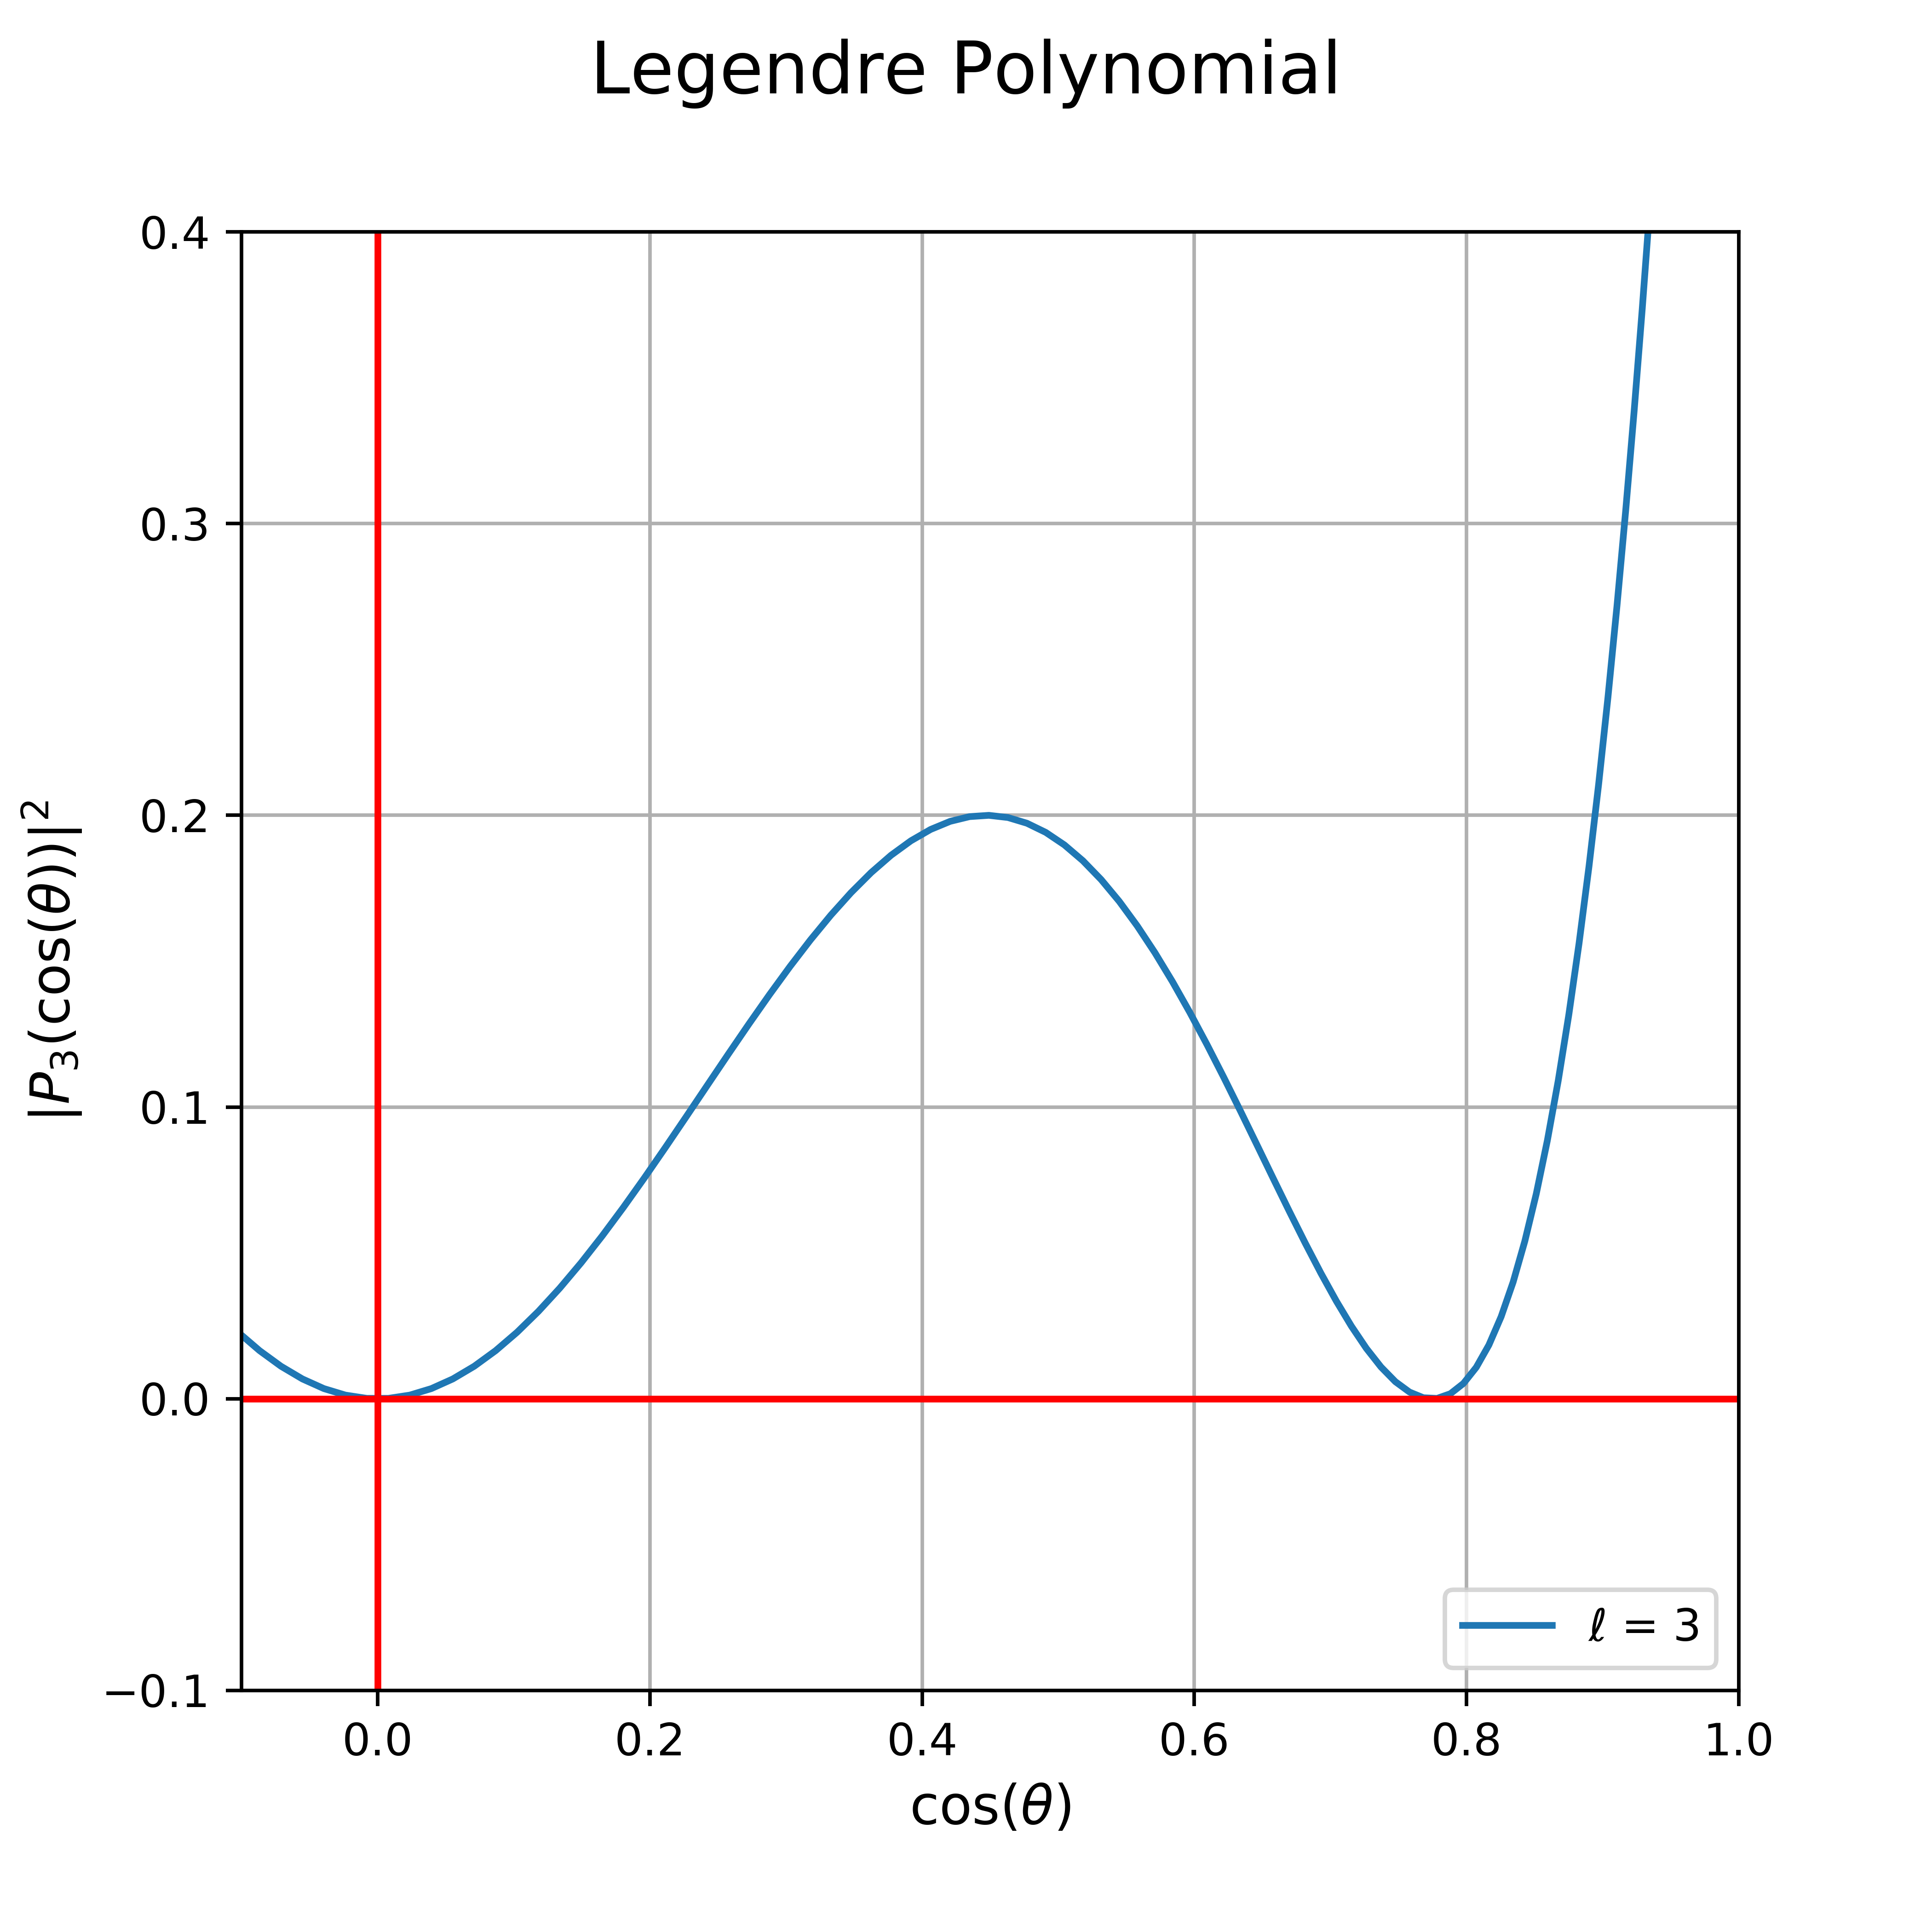
\includegraphics[height=6cm]{Legendre/legendreL3.png}\label{L3}}
	\caption{Comparison of the measured data and the $\ell=3$ Legendre polynomial for the $4962$ Hz resonance.}
	\label{legendre3}
\end{figure}

\begin{figure}[H]
	\centering
	\subfloat[Measured acoustic amplitude plotted against $\cos(\theta)$ for the 6202 Hz resonance]{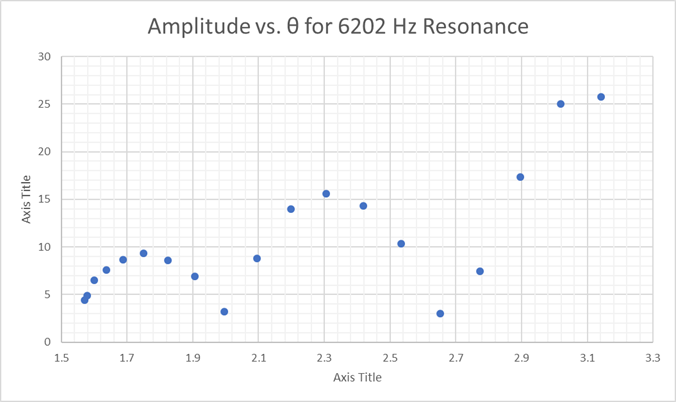
\includegraphics[height=6cm]{Graphs/6202Graph.png}}
	\qquad
	\subfloat[Legendre polynomial $|\mathrm{P}_4|^2$]{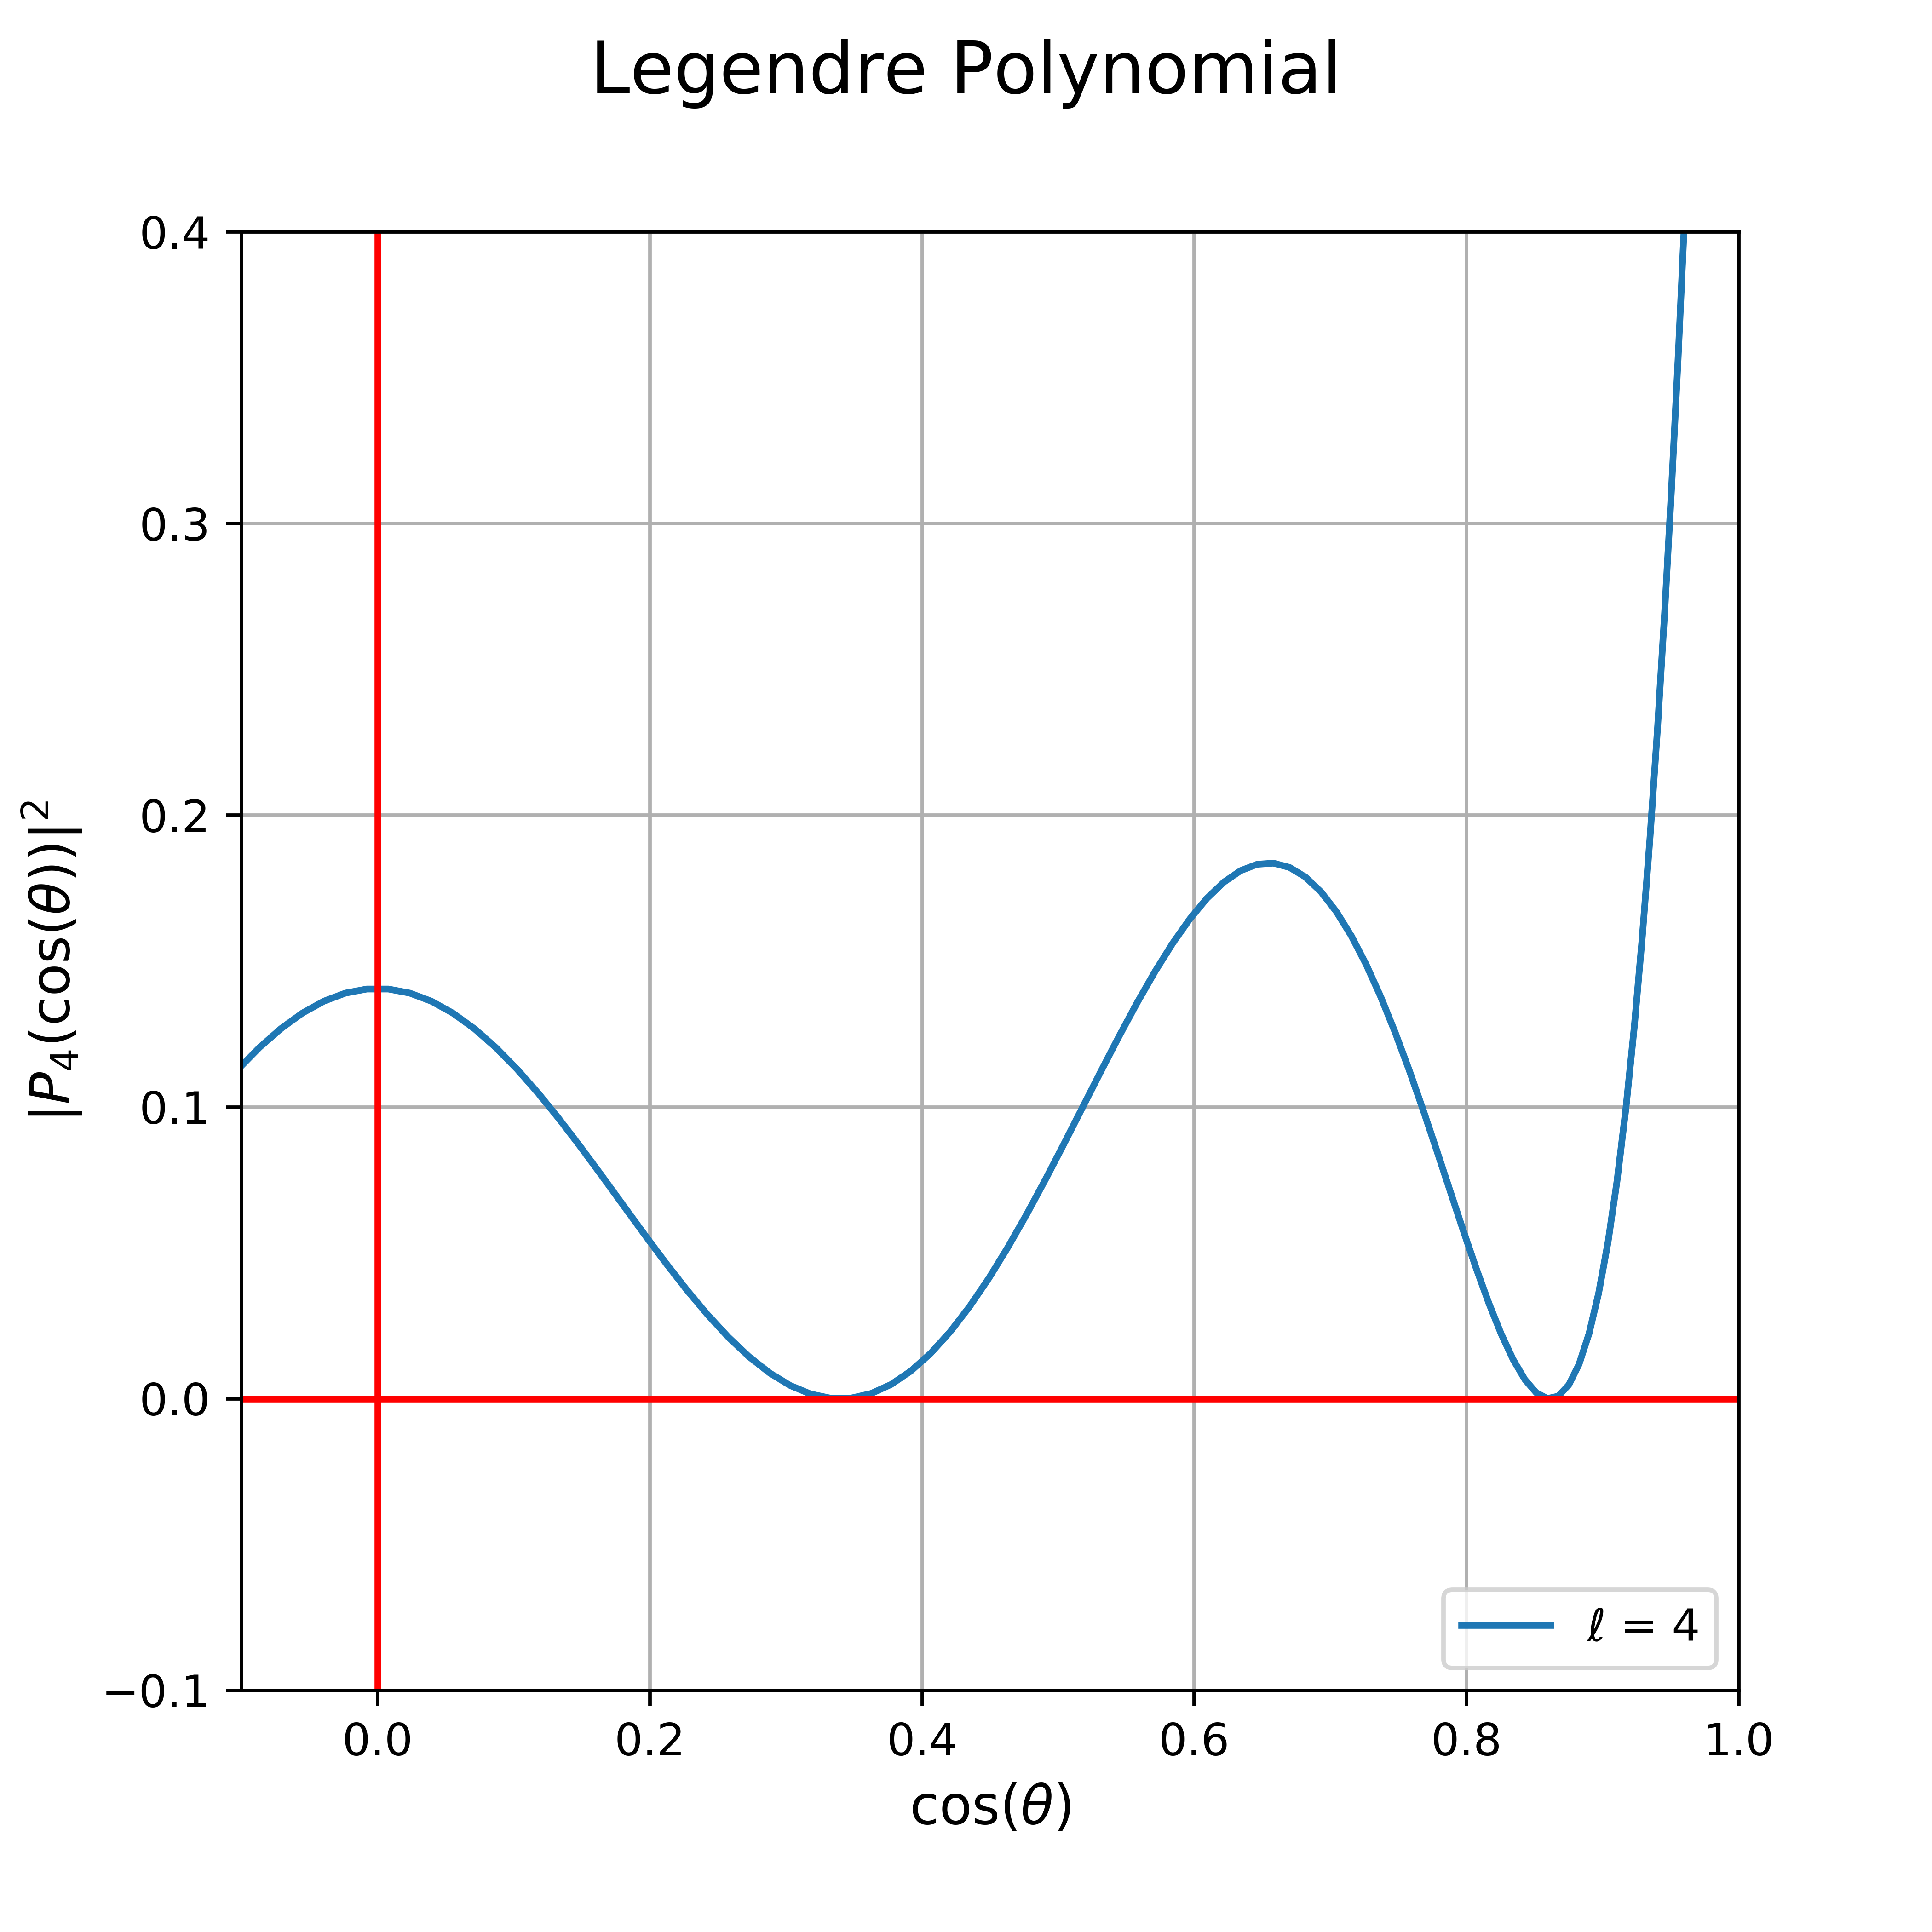
\includegraphics[height=6cm]{Legendre/legendreL4.png}\label{L4}}
	\caption{Comparison of the measured data and the $\ell=4$ Legendre polynomial for the $6202$ Hz resonance.}
	\label{legendre4}
\end{figure}

\begin{figure}[H]
	\centering
	\subfloat[Measured acoustic amplitude plotted against $\cos(\theta)$ for the 7409 Hz resonance]{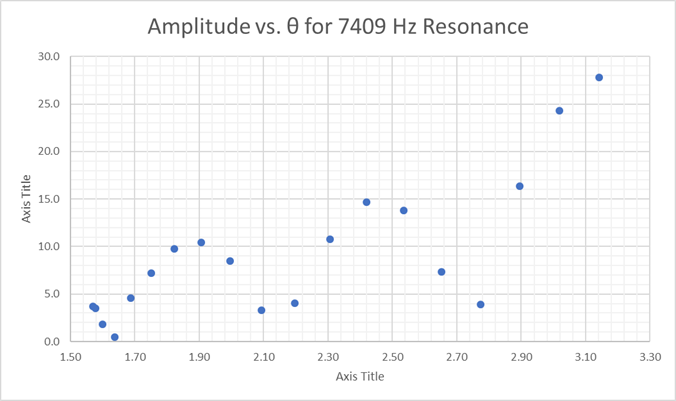
\includegraphics[height=6cm]{Graphs/7409Graph.png}}
	\qquad
	\subfloat[Legendre polynomial $|\mathrm{P}_5|^2$]{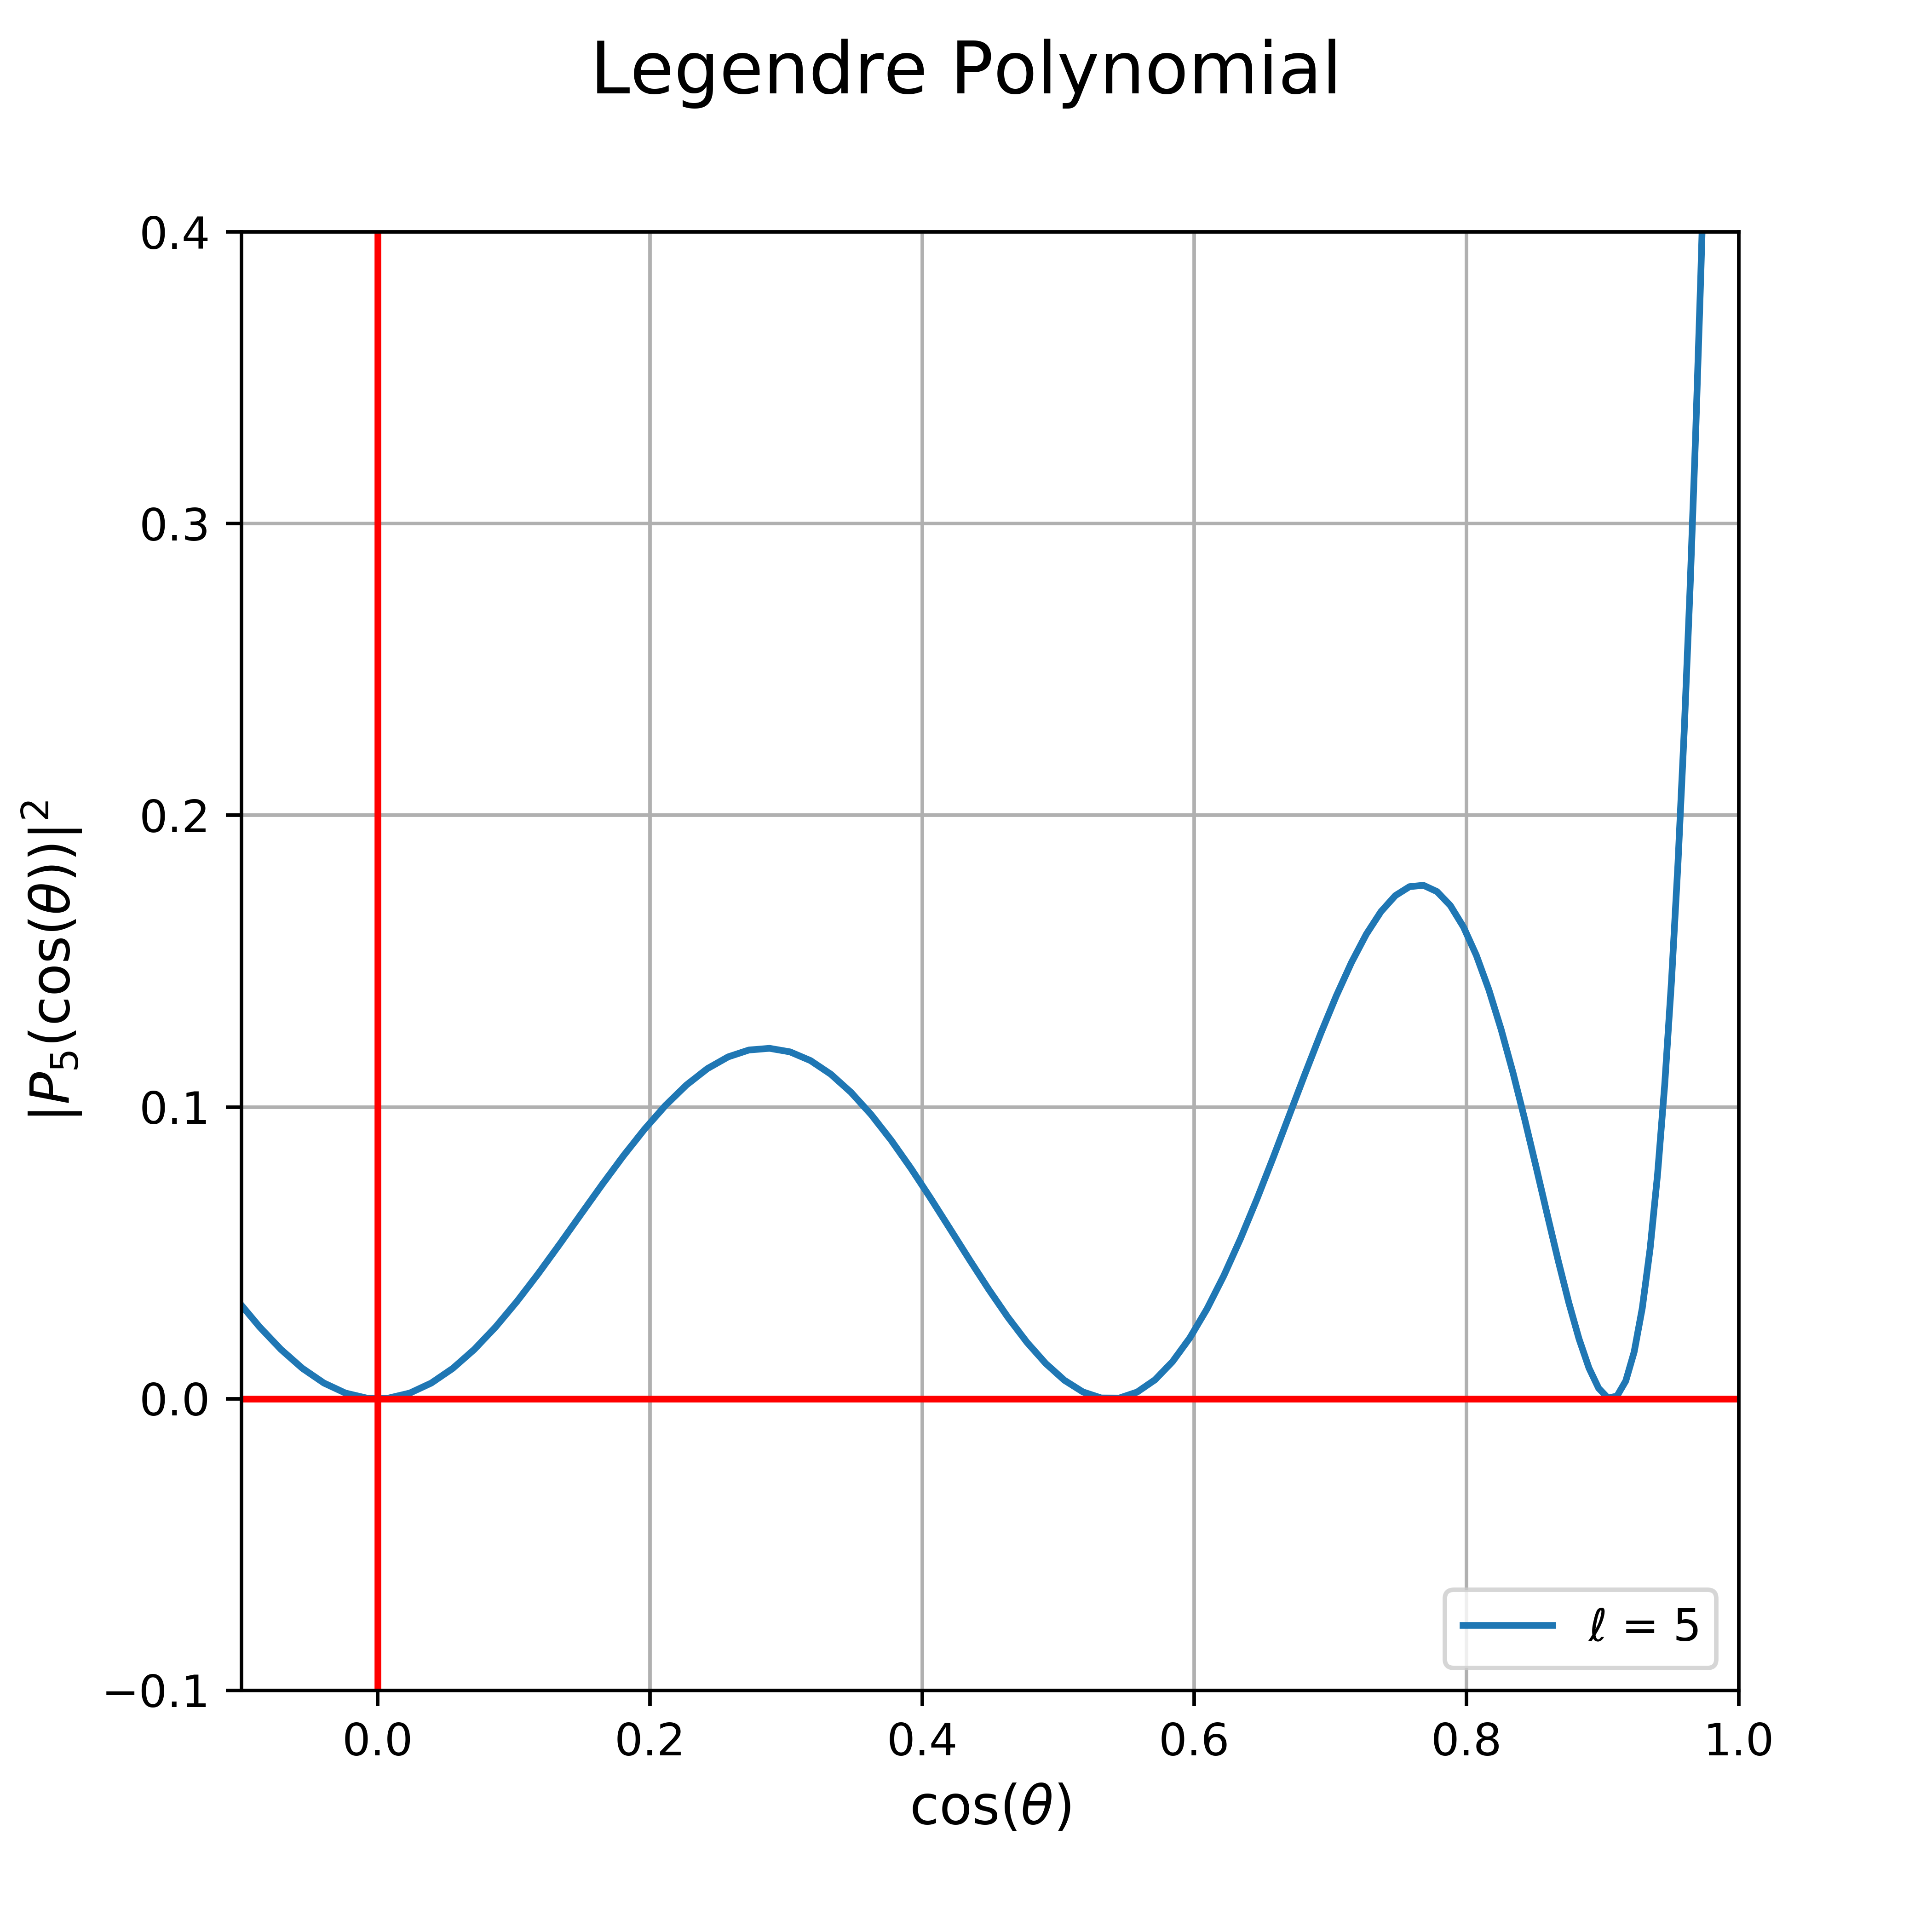
\includegraphics[height=6cm]{Legendre/legendreL5.png}\label{L5}}
	\caption{Comparison of the measured data and the $\ell=5$ Legendre polynomial for the $7409$ Hz resonance.}
	\label{legendre5}
\end{figure}

\subsection{Spherical Harmonics}


\begin{figure}[H]
	\centering
	\subfloat[$\ell=1$, $m=0$ polar plot for 2291 Hz resonance]{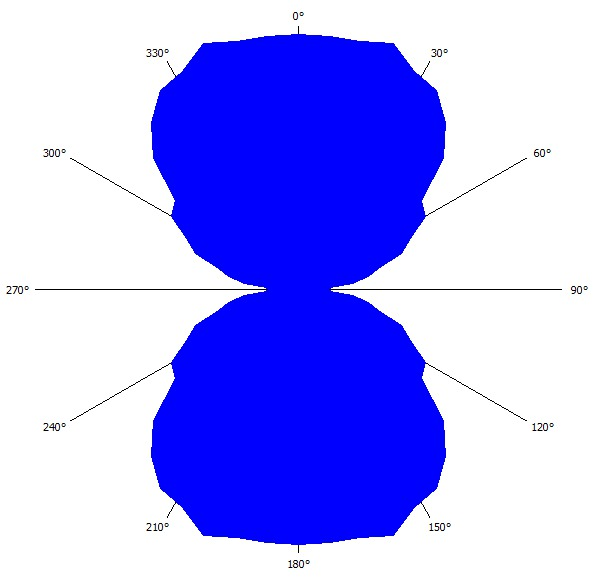
\includegraphics[width=0.35\textwidth]{2.3.2/F2291.jpg}\label{Polar2291}}
	\qquad \qquad
	\subfloat[$\ell=2$, $m=0$  plot for 3679 Hz resonance ]{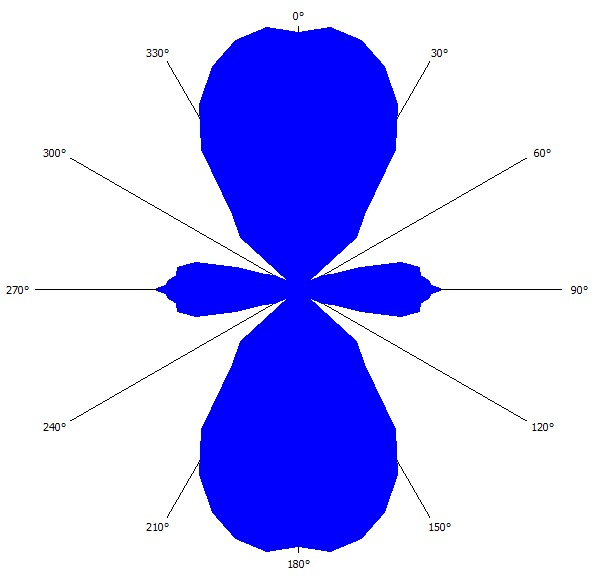
\includegraphics[width=0.35\textwidth]{2.3.2/F3679.jpg}\label{Polar3679}}
	\\
	\subfloat[$\ell=3$, $m=0$  plot for 4962 Hz resonance]{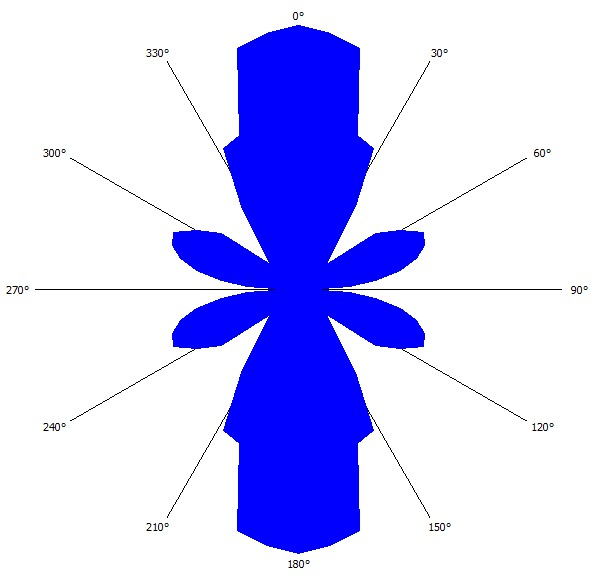
\includegraphics[width=0.35\textwidth]{2.3.2/F4962.jpg}\label{Polar4962}}
	\qquad \qquad
	\subfloat[$\ell=5$, $m=0$  plot for 7409 Hz resonance]{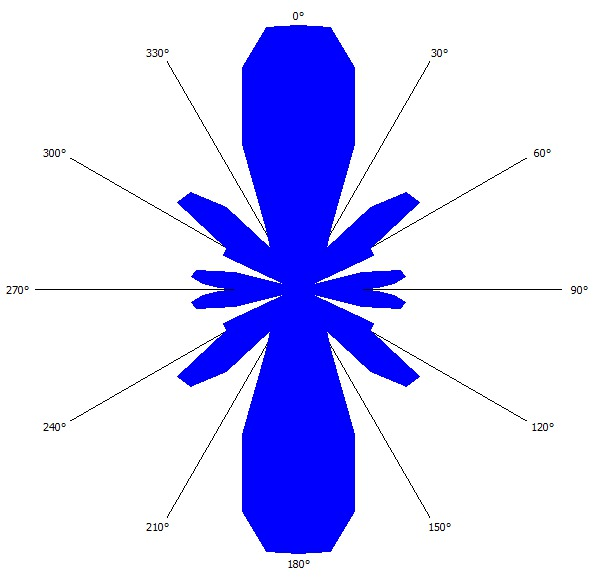
\includegraphics[width=0.35\textwidth]{2.3.2/F7409.jpg}\label{Polar6202}}
	\caption{Acoustic amplitude vs polar angle ($\theta$) with azimuthal angle $\varphi = 0$ for 4 resonant frequencies. Comparing these to the spherical harmonics in \figref{sphereHarm}, it is possible to determine the angular momentum quantum number $\ell$ for each resonance.}
	\label{polarGraphs}
\end{figure}

\begin{figure}[H]
	\centering
	\subfloat[Spherical harmonic for $\ell = 1$, $m= 0$]{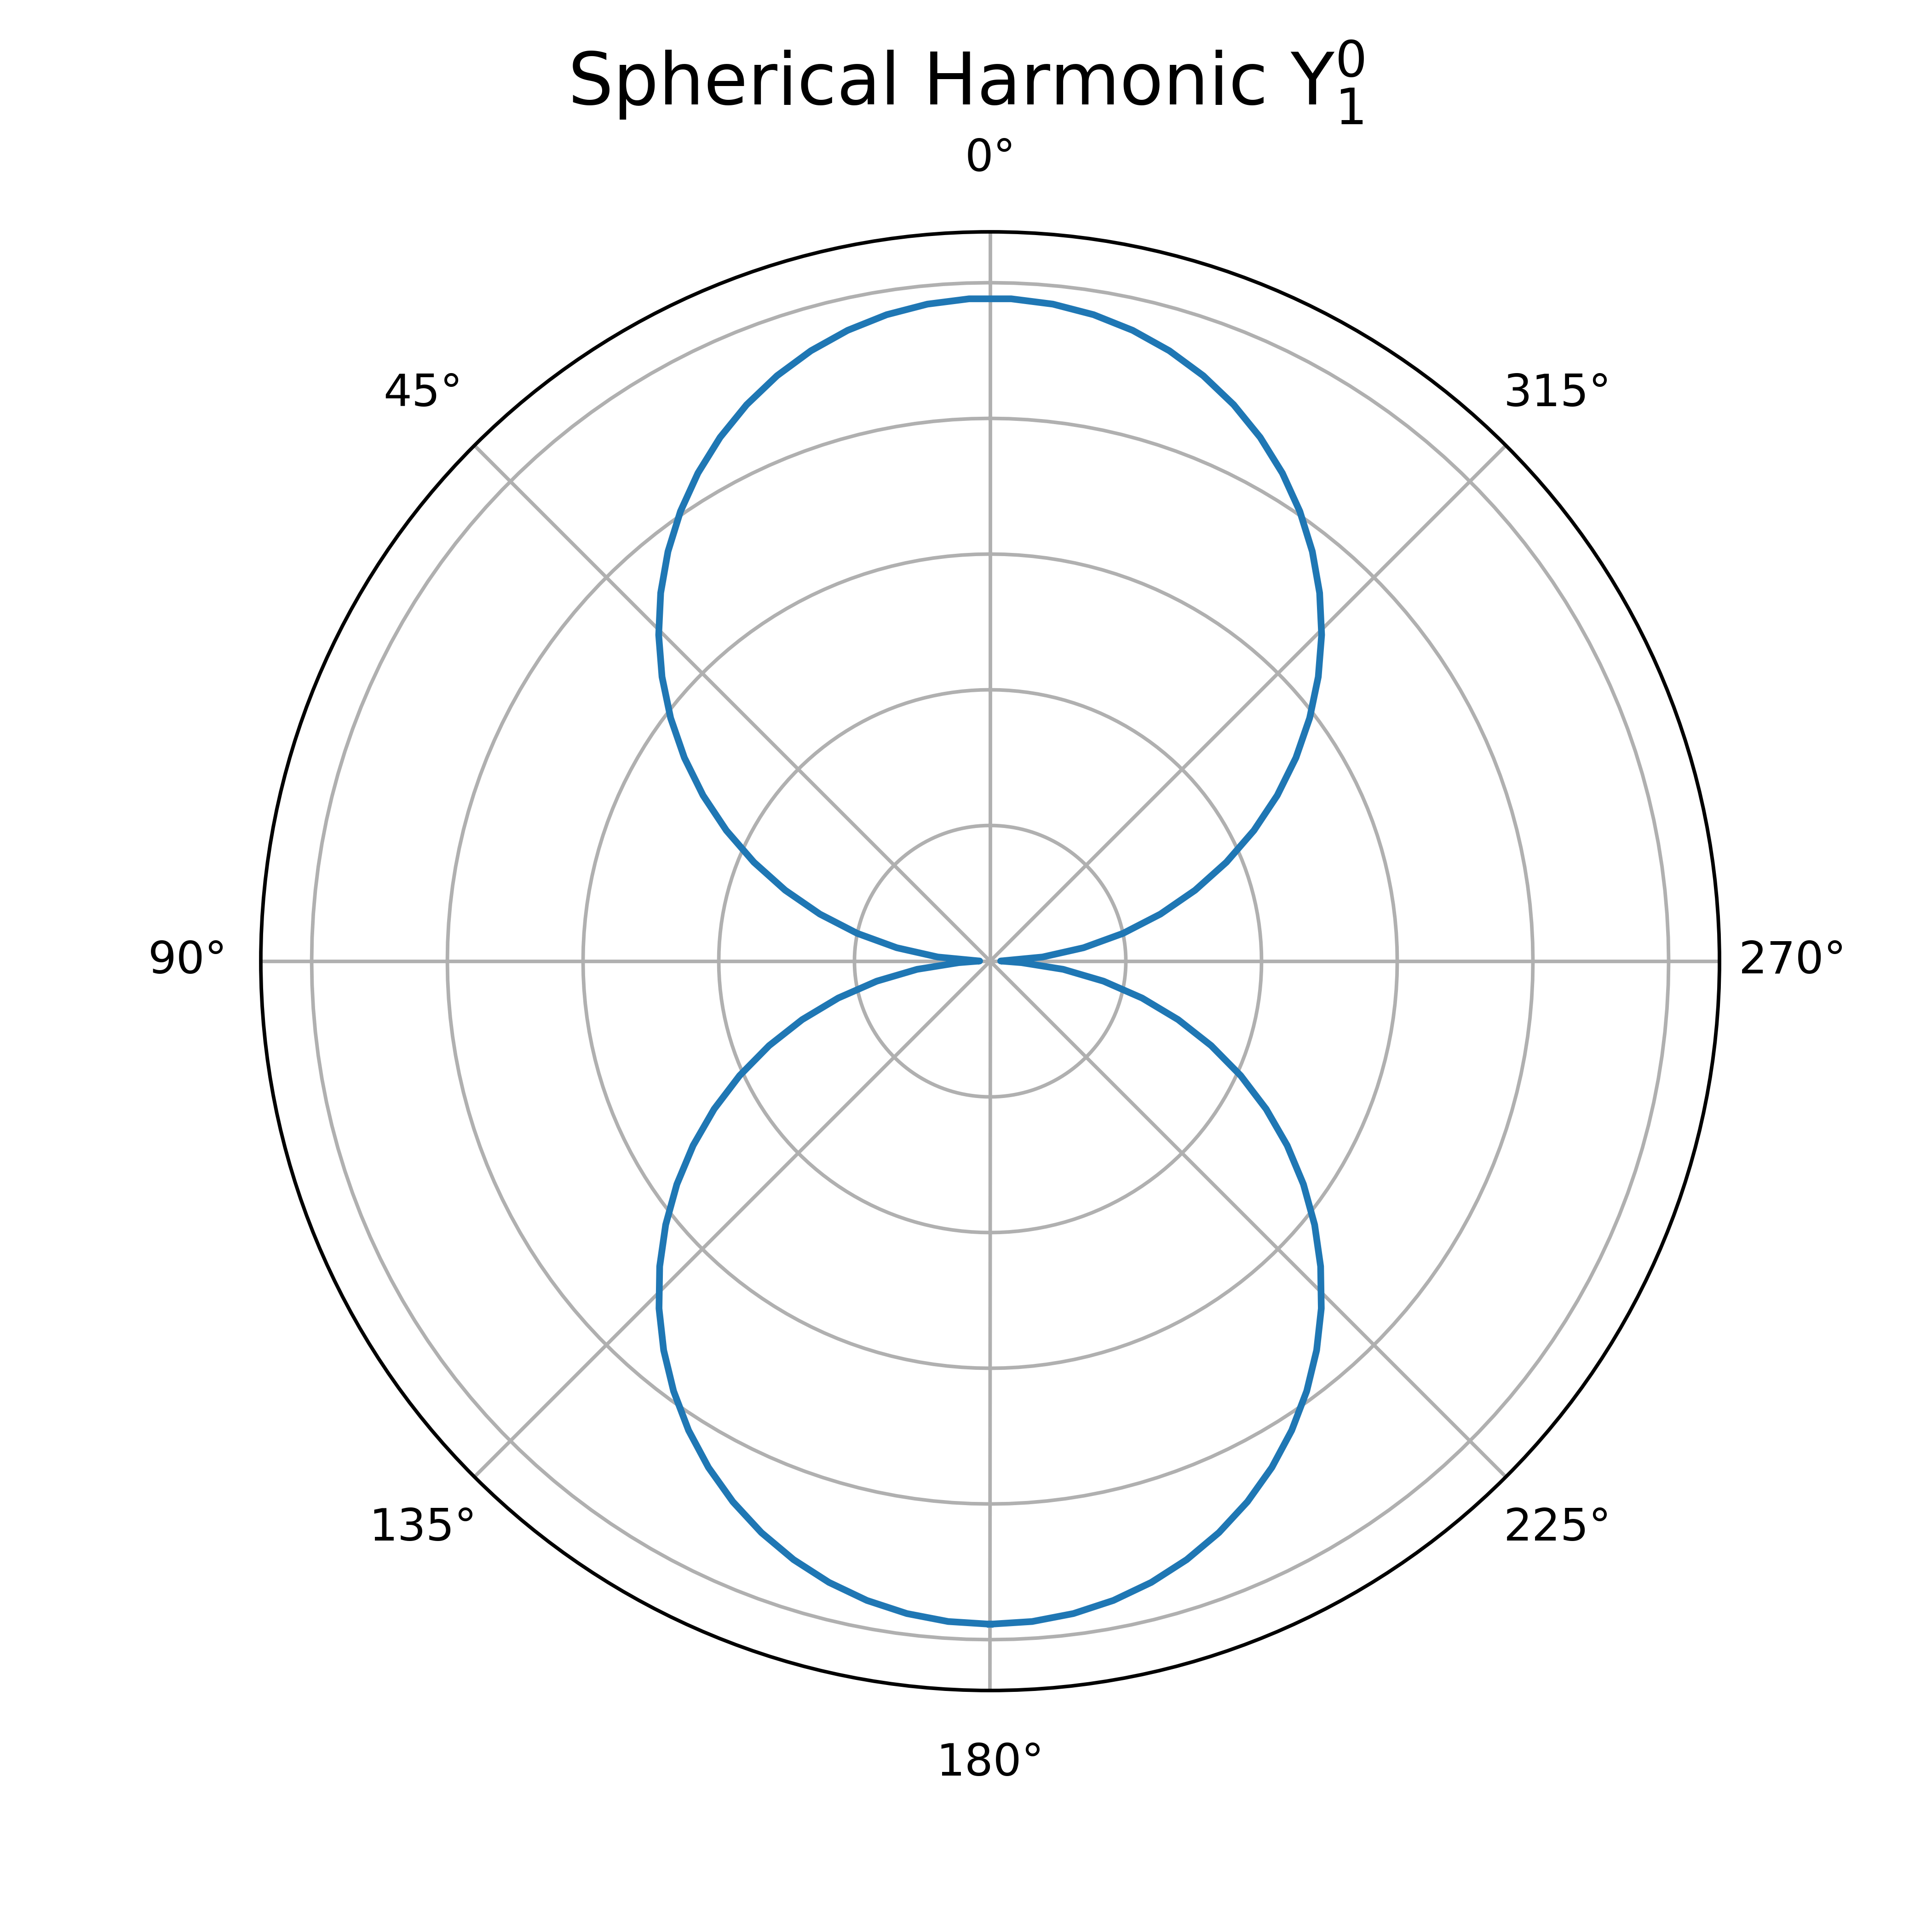
\includegraphics[width=0.4\textwidth]{SphHarm/SphHarmL1M0.png}\label{sphHarmL1M0}}
	\qquad \quad
	\subfloat[Spherical harmonic for $\ell = 2$, $m=0$]{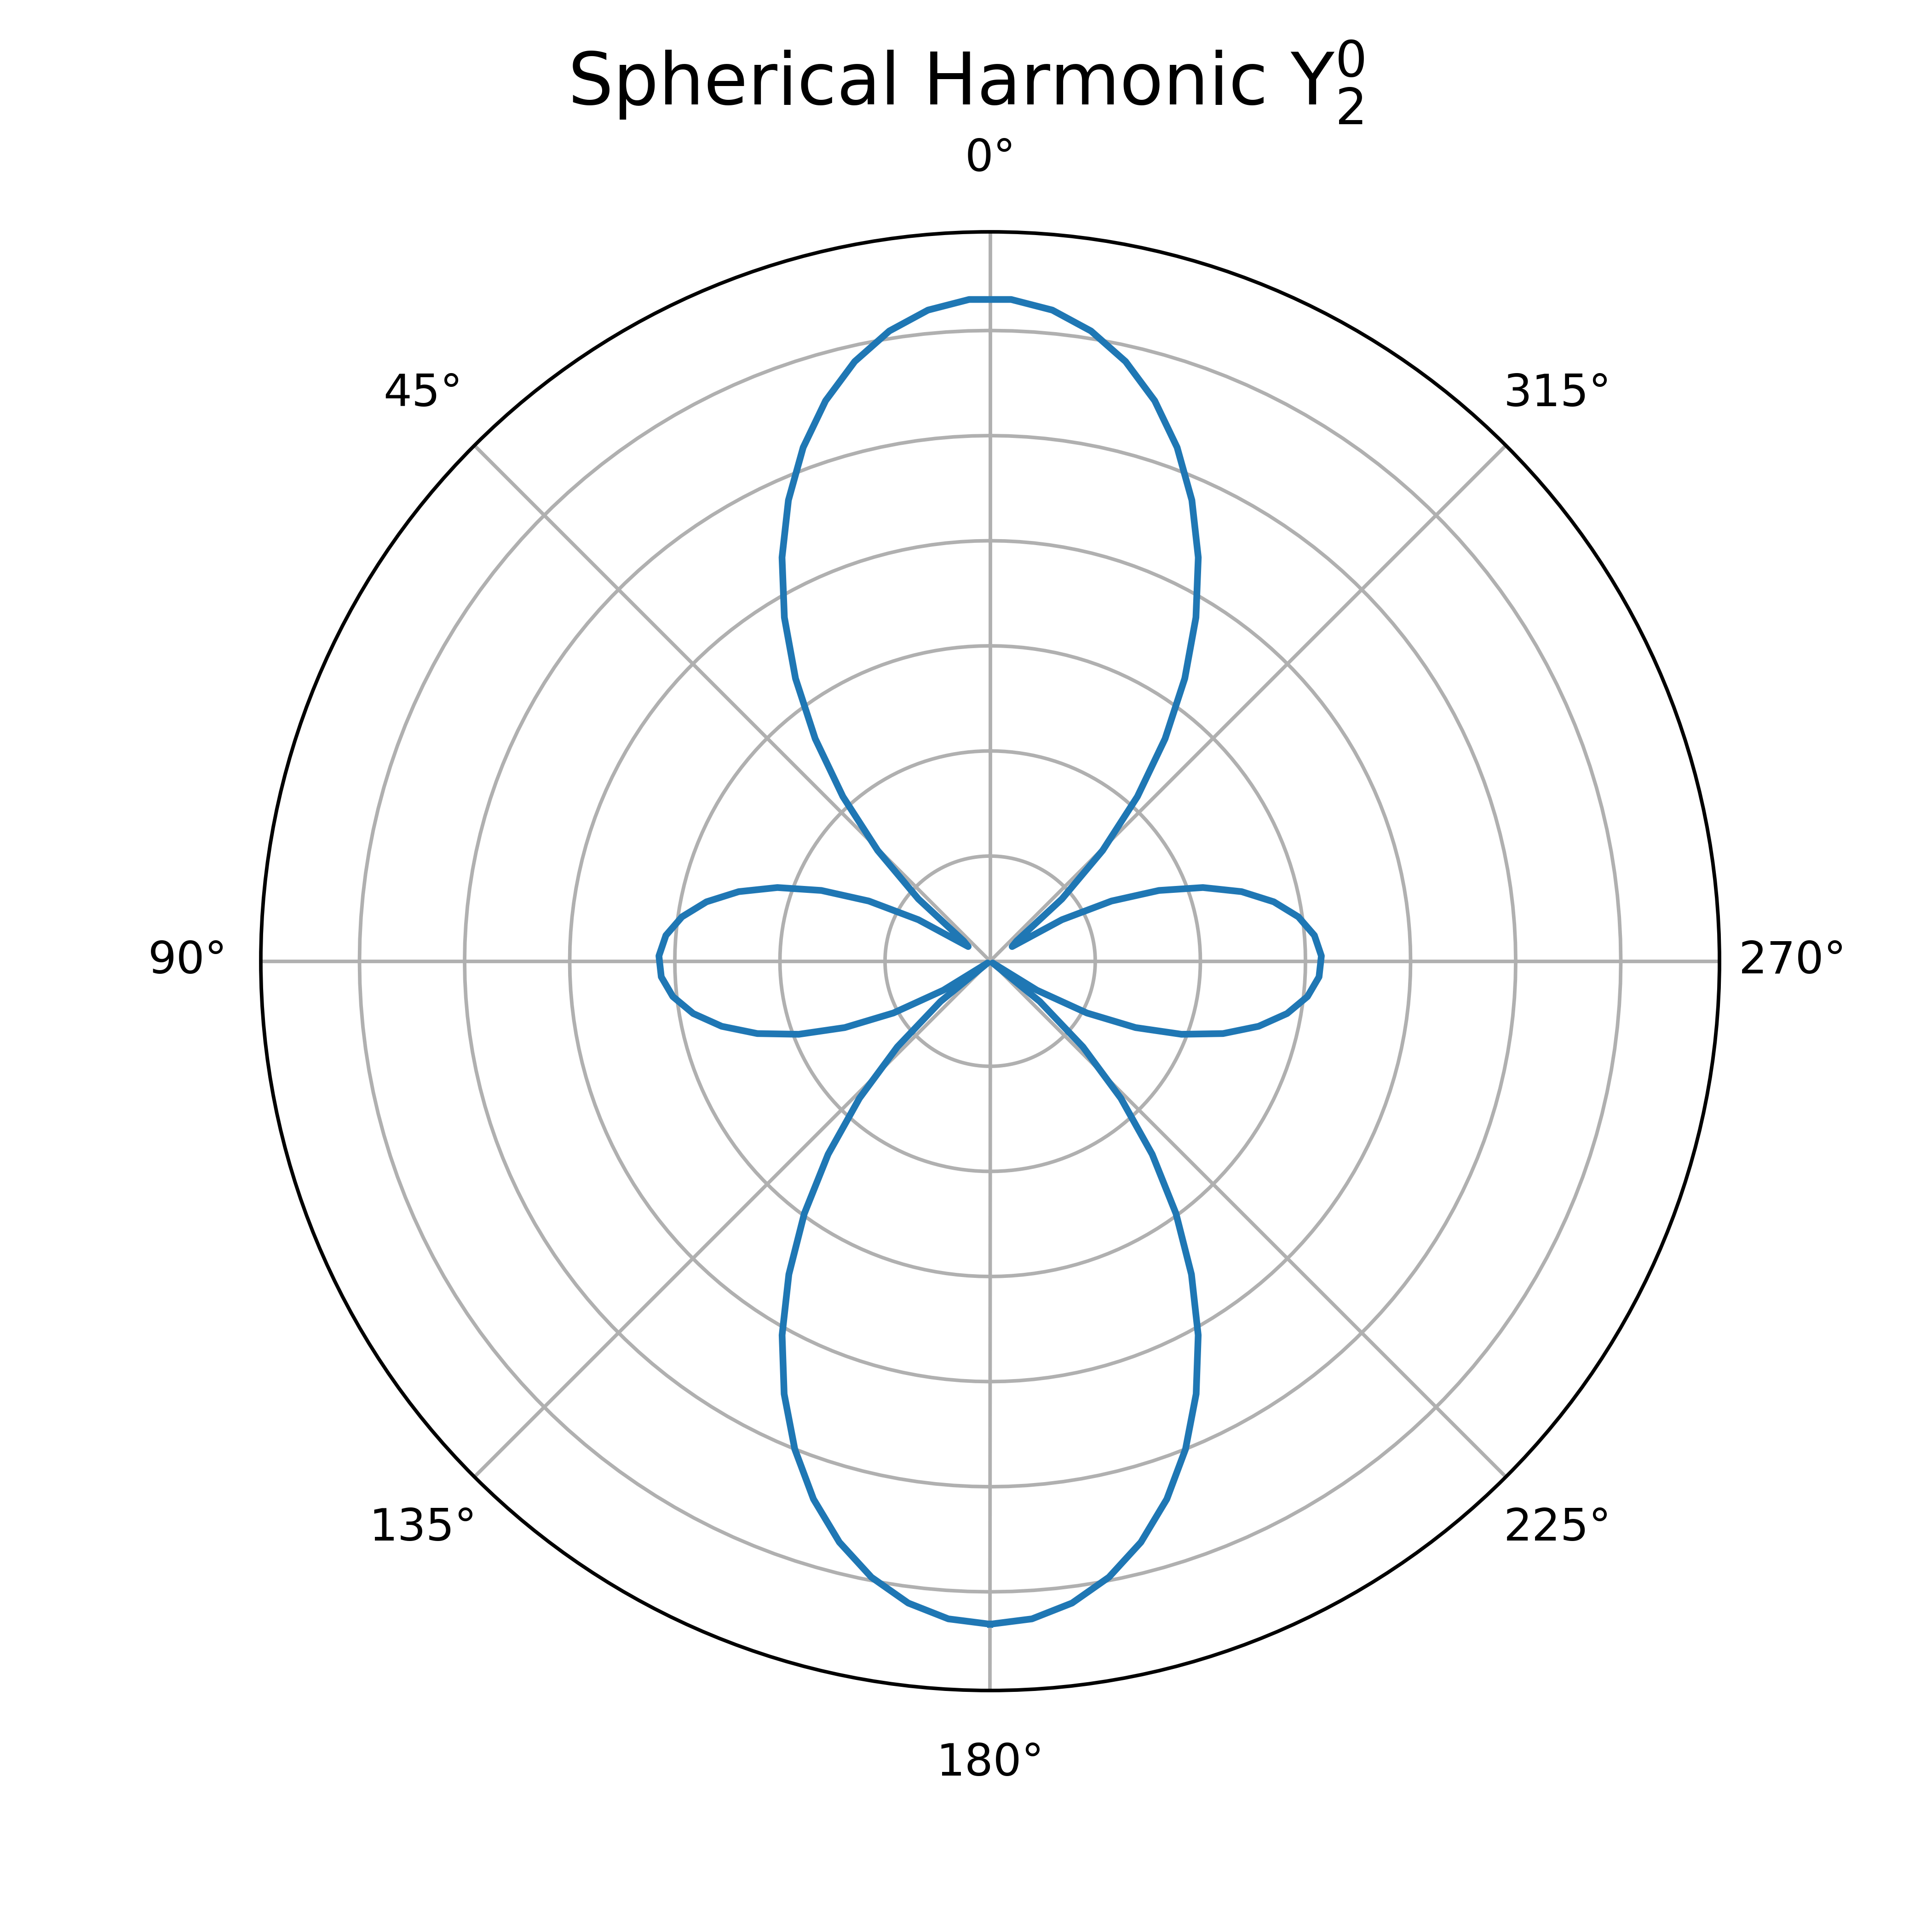
\includegraphics[width=0.4\textwidth]{SphHarm/SphHarmL2M0.png}\label{sphHarmL2M0}}
	\\
	\subfloat[Spherical harmonic for $\ell = 3$, $m = 0$]{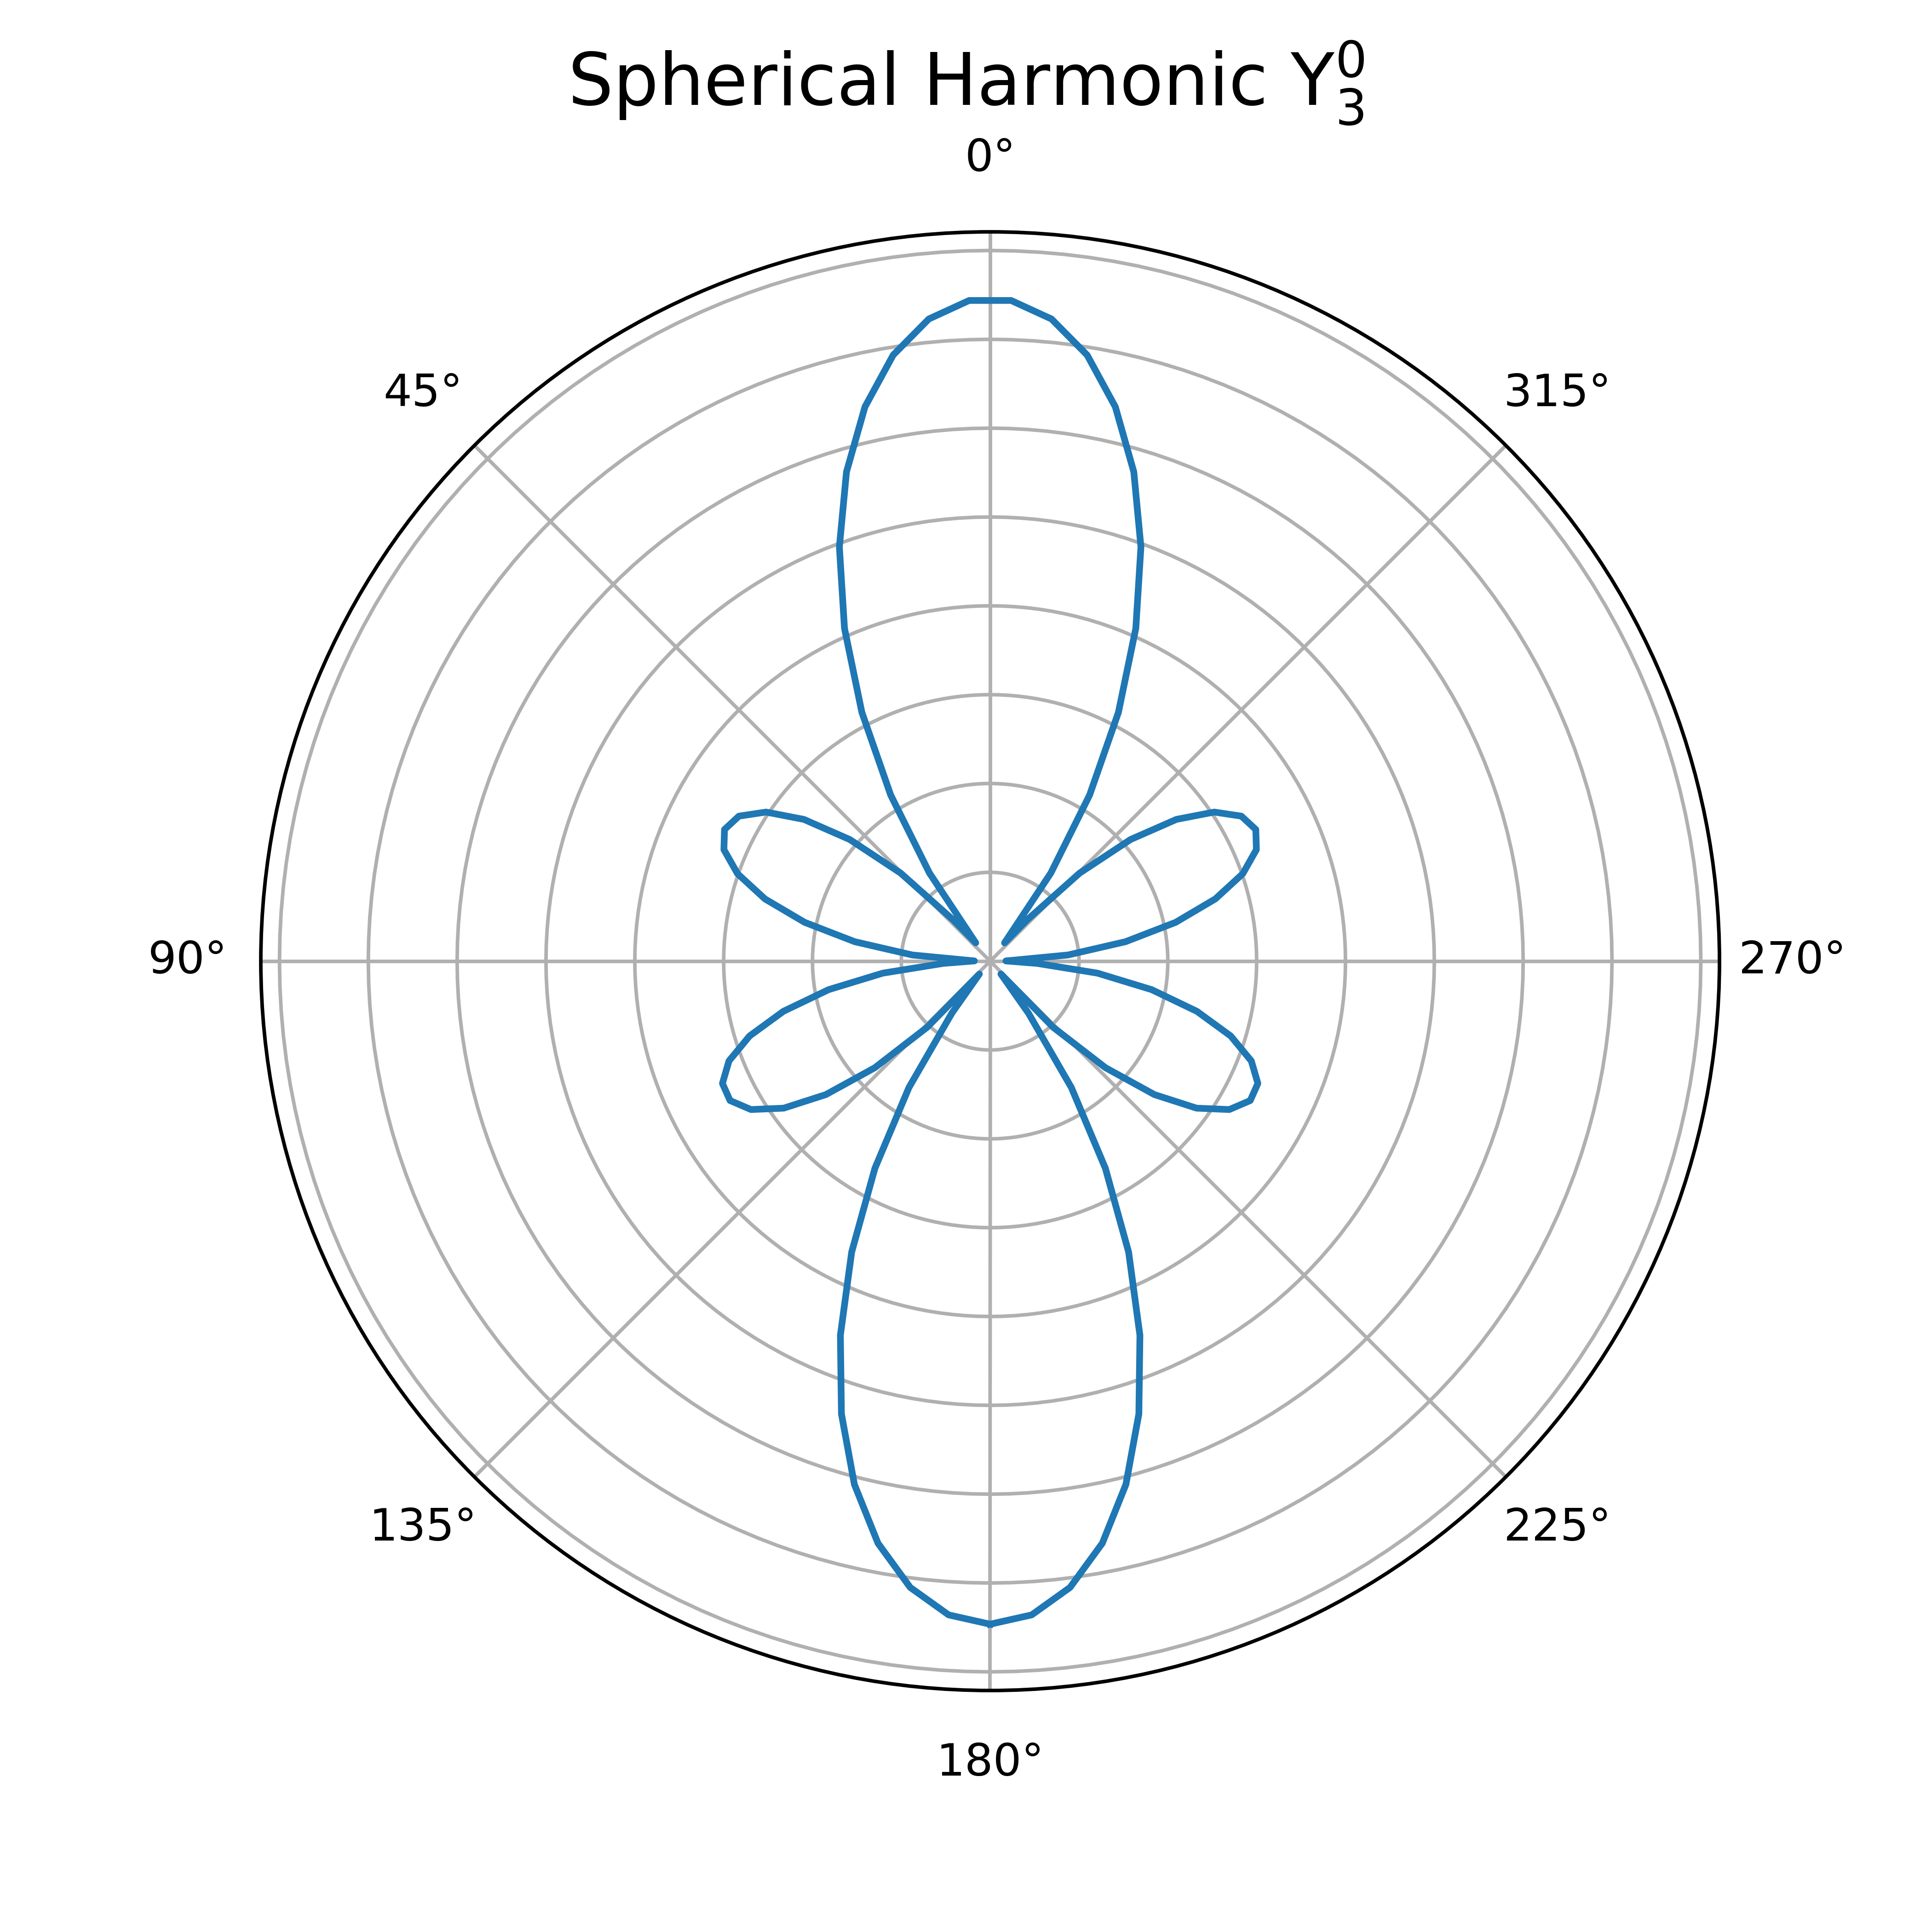
\includegraphics[width=0.4\textwidth]{SphHarm/SphHarmL3M0.png}\label{sphHarmL3M0}}
	\qquad \quad
	\subfloat[Spherical harmonic for $\ell = 5$, $m = 1$]{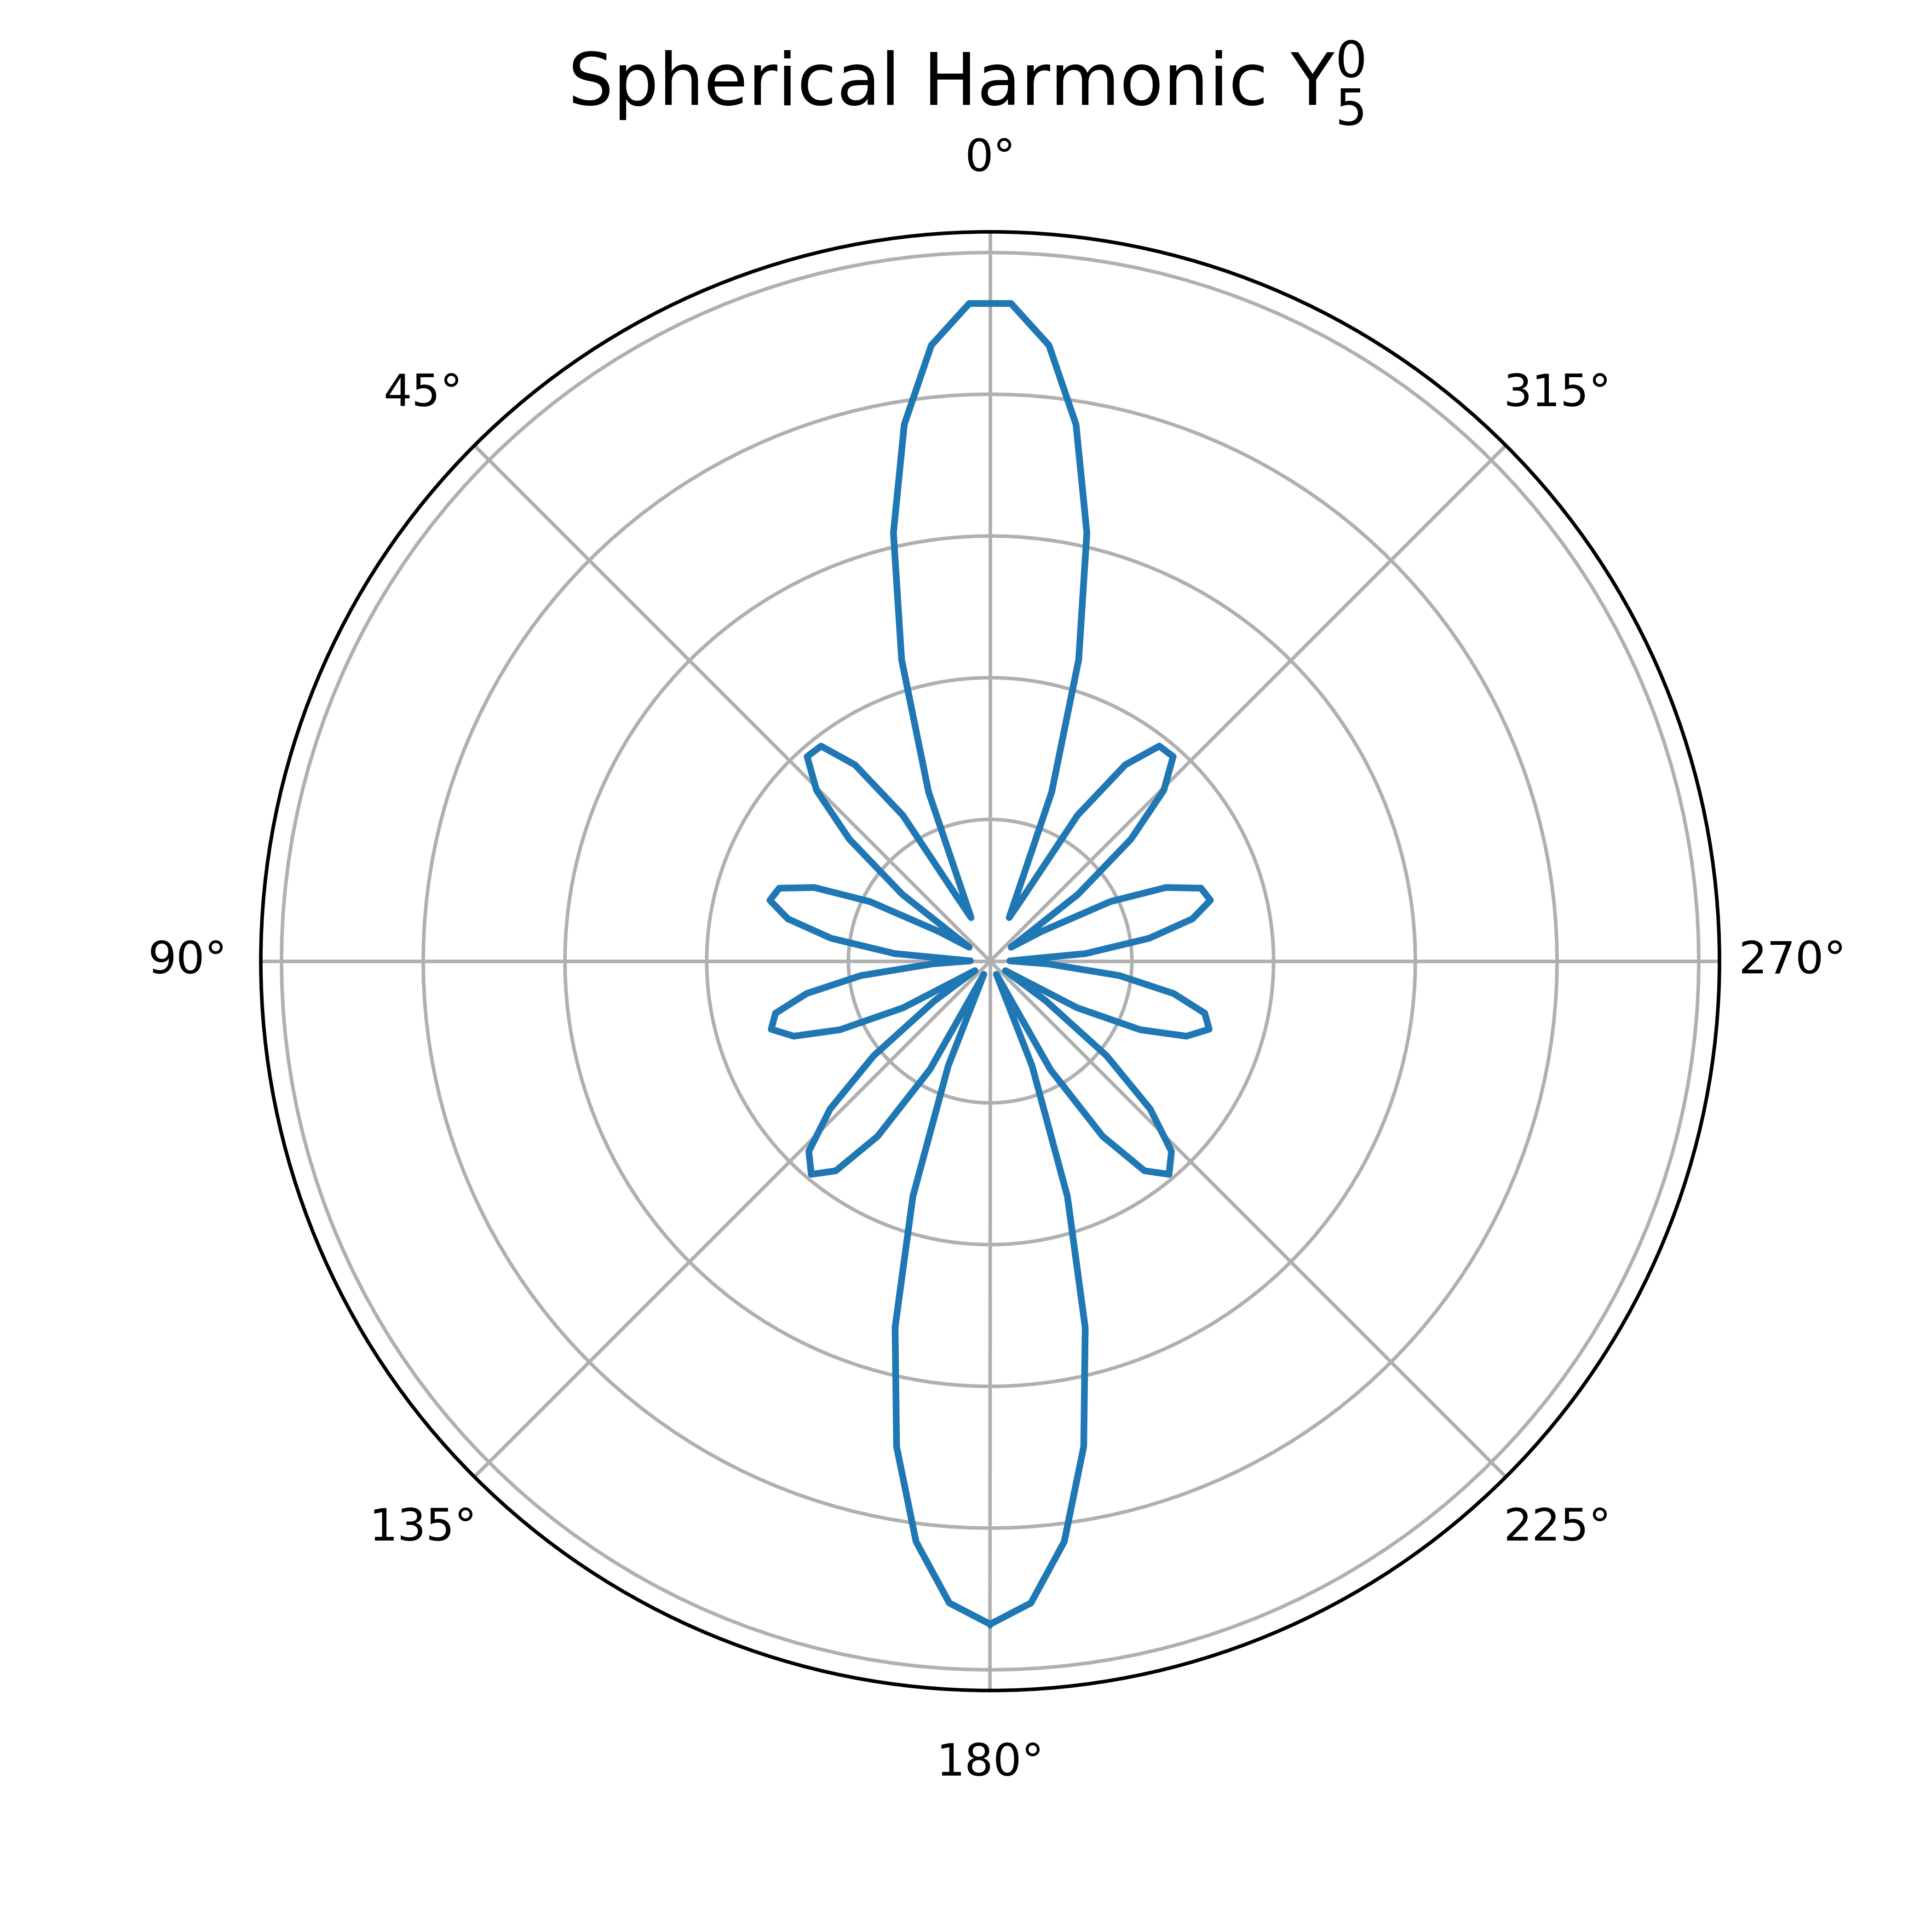
\includegraphics[width=0.4\textwidth]{SphHarm/SphHarmL5M0.png}\label{sphHarmL5M0}}
	\caption{Projections of the spherical harmonics $\mathrm{Y}^\ell_m$ onto the $\varphi = 0$ plane. Angle markings indicate polar angle $\theta$.}
	\label{sphereHarm}
\end{figure}

\subsection{Polar Graphs with Broken Cavity Symmetry}


\begin{figure}[H]
	\captionsetup{justification = centering}
	\centering
	\subfloat[$\ell=1$, $m=0$]{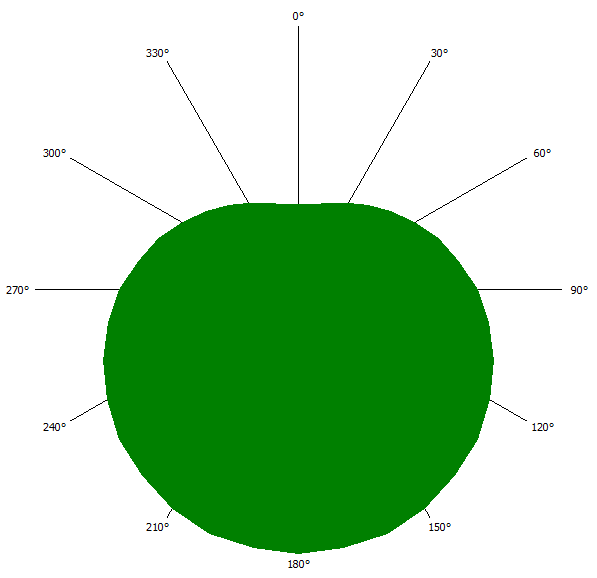
\includegraphics[width=0.35\textwidth]{Day4/L13mmPolar2084_806.png}}
	\qquad \quad
	\subfloat[$\ell=1$, $m=\pm1$]{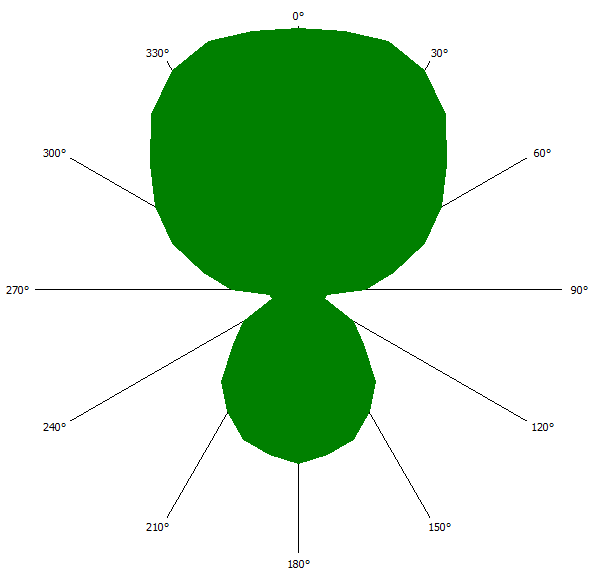
\includegraphics[width=0.35\textwidth]{Day4/L13mmPolar2251_140.png}}
	\caption{Amplitude versus polar angle $\theta$ for the $\ell=1$ resonance with 3mm Spacing}
	\label{3mmliftedDegeneracy}
\end{figure}


\begin{figure}[H]
	\captionsetup{justification = centering}
	\centering
	\subfloat[[$\ell=1$, $m=0$]{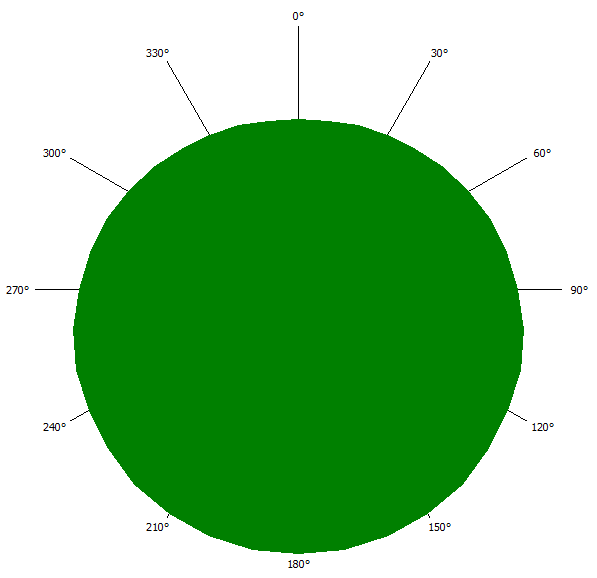
\includegraphics[width=0.35\textwidth]{Day4/L16mmPolar2084_806.png}}
	\qquad \quad
	\subfloat[[$\ell=1$, $m=\pm1$]{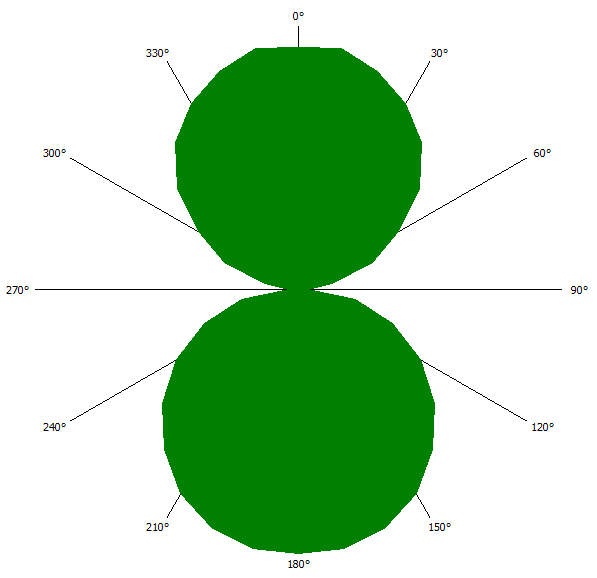
\includegraphics[width=0.35\textwidth]{Day4/L16mmPolar2251_140.png}}
	\caption{Amplitude versus polar angle $\theta$ for the $\ell=1$ resonance with 6mm Spacing}
	\label{6mmliftedDegeneracy}
\end{figure}

We can see that as the cavity separation is increased, simulating a stronger magnetic field, the shapes of the orbitals becomes more symmetric.


%	\begin{figure}[H]
%		\centering
%		\subfloat[$\ell=2$, $m=-1$ resonance]{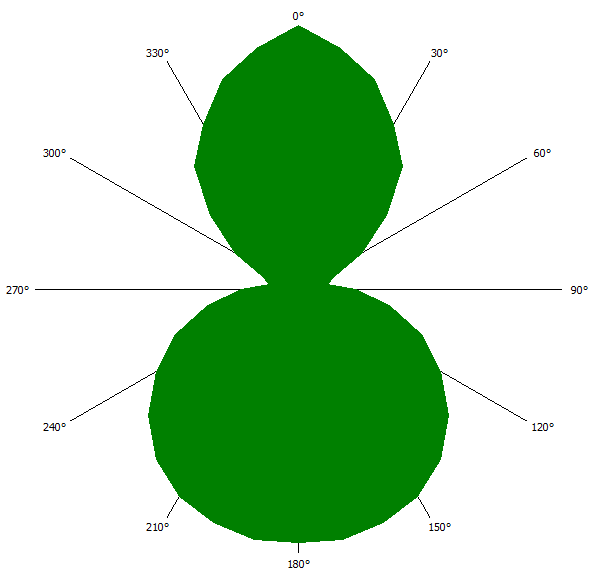
\includegraphics[width=0.3\textwidth]{2.3.3/3mmPolar/323_Polar_L1M-1Amp_freq3591_549.png} \label{3-0mmDegeneracy}}
%		\quad
%		\subfloat[$\ell=2$, $m=0$ resonance]{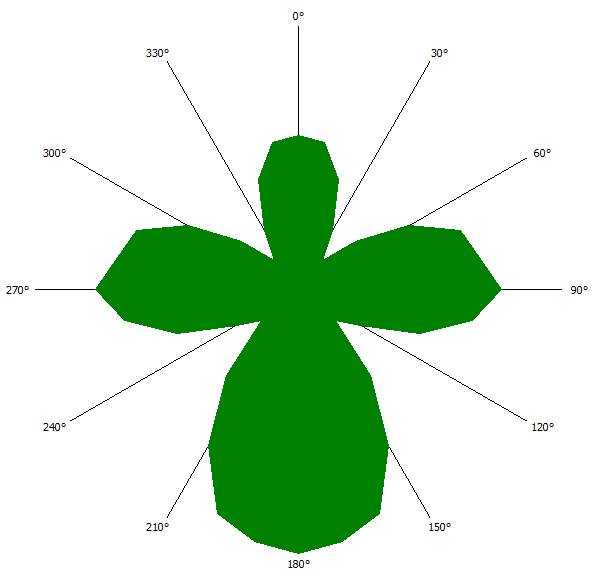
\includegraphics[width=0.3\textwidth]{2.3.3/3mmPolar/323_Polar_L1M1Amp_freq3647_513.png} \label{3-1mmDegeneracy}}
%		\caption{Polar plots of lifted degeneracies for 3mm spacing}
%		\label{3mmliftedDegeneracy}
%	\end{figure}
%	It is important to note that not all the degeneracies were lifted at $3$ mm spacing.


%
%	\begin{figure}[H]
%		\centering
%		\subfloat[$\ell=1$, $m=-1$ resonance]{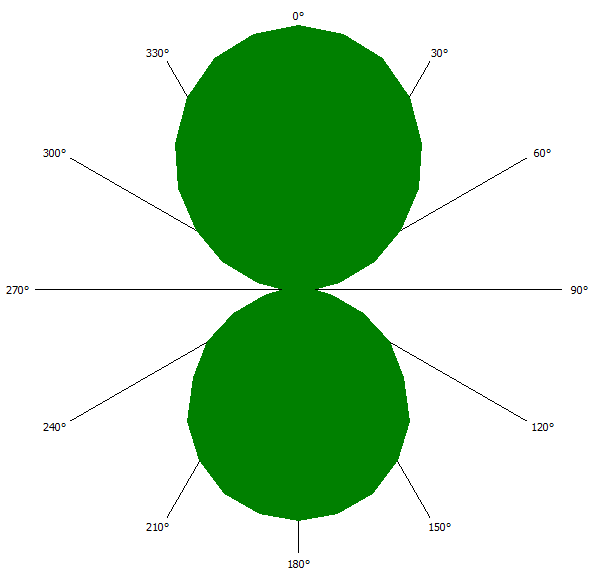
\includegraphics[width=0.3\textwidth]{2.3.3/6mmPolar/323_Polar_L1M-1Amp_freq3519_864.png} \label{6-m1mmDegeneracy}}
%		\quad
%		\subfloat[$\ell=1$, $m=0$ resonance]{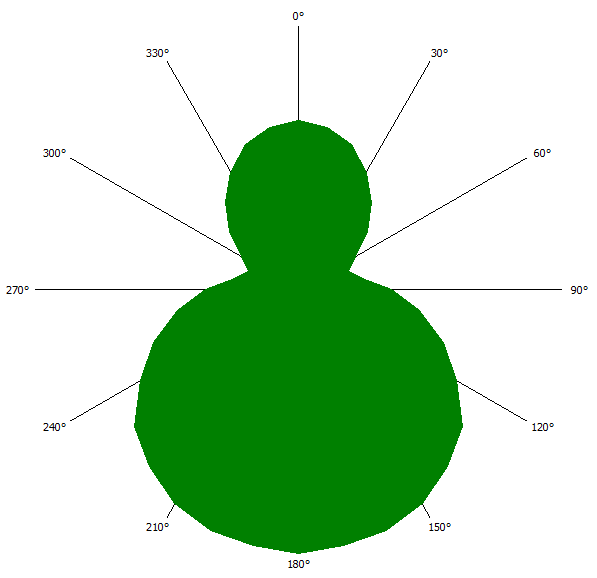
\includegraphics[width=0.3\textwidth]{2.3.3/6mmPolar/323_Polar_L1M0Amp_freq3534_956.png} \label{6-0mmDegeneracy}}
%		\quad
%		\subfloat[$\ell=1$, $m=1$ resonance]{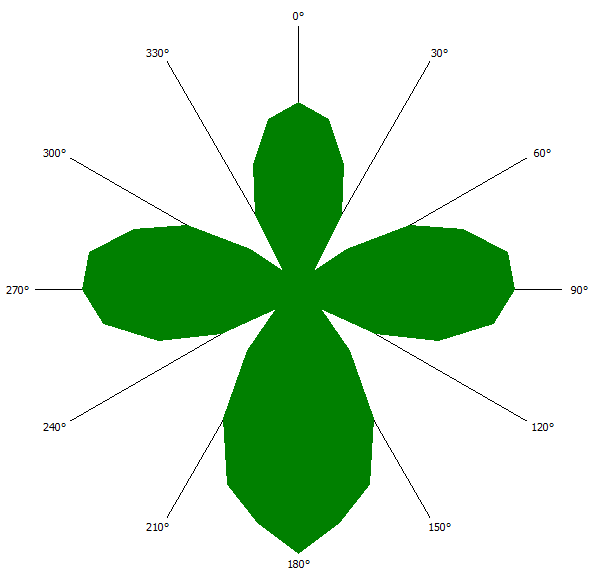
\includegraphics[width=0.3\textwidth]{2.3.3/6mmPolar/323_Polar_L1M1Amp_freq3632_422.png} \label{6-1mmDegeneracy}}
%		\caption{Polar plots of lifted degeneracies for 6mm spacing.}
%		\label{6mmliftedDegeneracy}
%	\end{figure}
%	
%	
%		Further, we focus on the \red{$\ell=2$} resonance and apply the spacing rings again to see how the peak splits.
%	
%	\begin{figure}[H]
%		\centering
%		\subfloat[Lifted degeneracy spectrum for $\ell=2$ 3mm spacing]{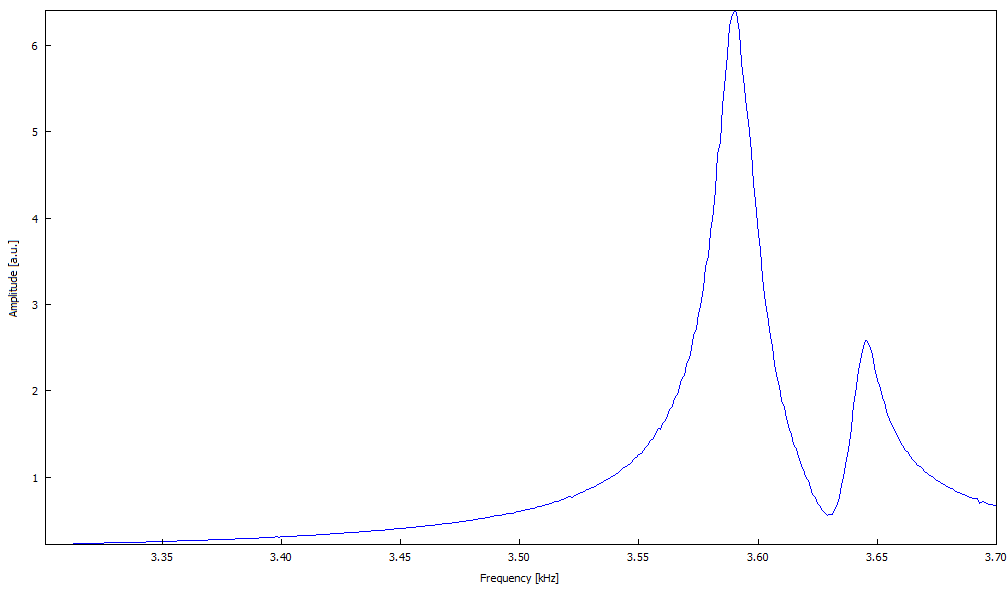
\includegraphics[width=0.3\textwidth]{2.3.3/323a180L13mmHires.png} \label{3mmDegeneracySpectrum}}
%		\quad
%		\subfloat[Lifted degeneracy spectrum for $\ell=2$ 6mm spacing]{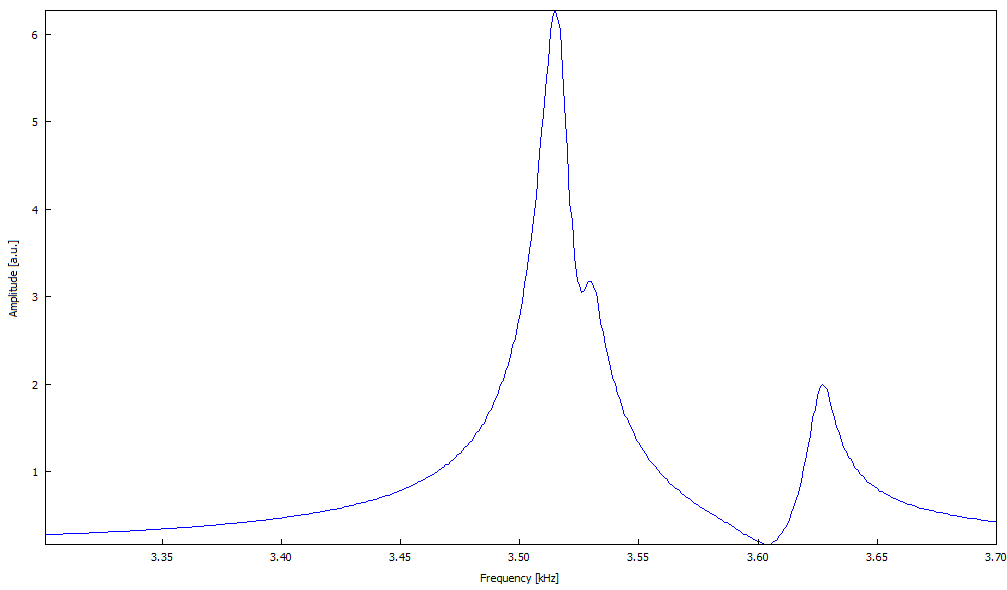
\includegraphics[width=0.3\textwidth]{2.3.3/323a180L16mmHires.png} \label{6mmDegeneracySpectrum}}
%		\quad
%		\subfloat[Lifted degeneracy spectrum for $\ell=2$ 9mm spacing]{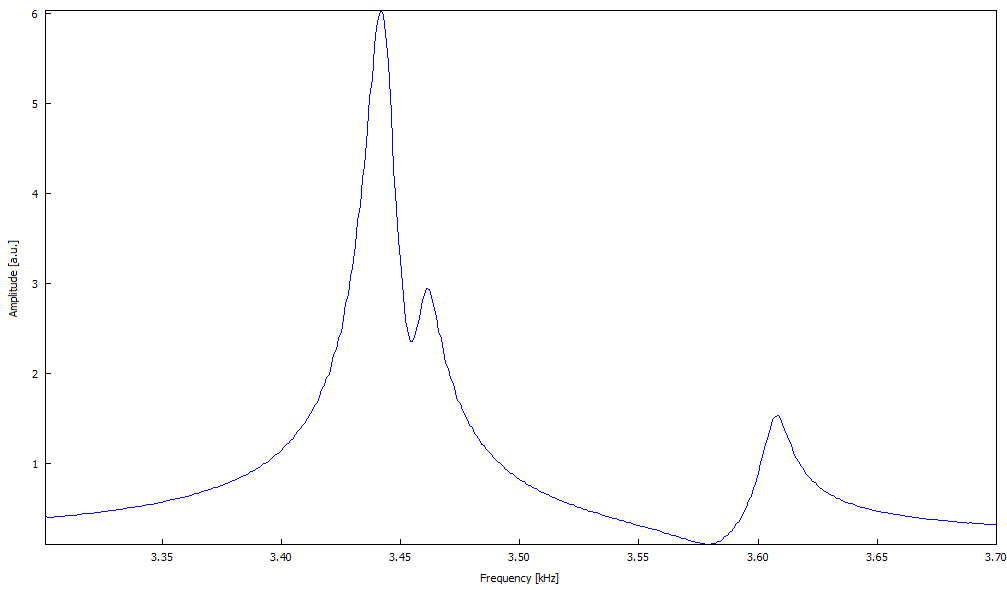
\includegraphics[width=0.3\textwidth]{2.3.3/323a180L19mmHires.png} \label{9mmDegeneracySpectrum}}
%		\caption{Progression of lifted degeneracies for the \red{$\ell=2$} state.}
%		\label{liftedDegeneracySpectrum}
%	\end{figure}